%# -*- coding: utf-8-unix -*-
%%==================================================
%% thesis.tex
%%==================================================

% 双面打印
% \documentclass[doctor, fontset=adobe, openright, twoside, zihao=-4]{sjtuthesis}
\documentclass[master, fontset=adobe, openany, oneside, submit, zihao=-4]{sjtuthesis} 
% \documentclass[master, adobefonts, review]{sjtuthesis} 
% \documentclass[%
%   bachelor|master|doctor,	% 必选项
%   fontset=adobe|windows,  	% 只测试了adobe
%   oneside|twoside,		% 单面打印,双面打印(奇偶页交换页边距,默认)
%   openany|openright, 		% 可以在奇数或者偶数页开新章|只在奇数页开新章(默认)
%   zihao=-4|5,, 		% 正文字号:小四、五号(默认)
%   review,	 		% 盲审论文,隐去作者姓名、学号、导师姓名、致谢、发表论文和参与的项目
%   submit			% 定稿提交的论文,插入签名扫描版的原创性声明、授权声明 
% ]

\begin{document}

%% 无编号内容:中英文论文封面、授权页
%# -*- coding: utf-8-unix -*-
\title{有源配电网自适应方向保护研究}
\author{范忻蓉}
\advisor{张沛超}
% \coadvisor{某某教授}
\defenddate{2017年1月}
\school{上海交通大学}
\institute{电子信息与电气工程}
\studentnumber{1140369007}
\major{电力系统及其自动化}

\englishtitle{RESEARCH ON ADAPITIVE DIRECTIONAL PROTECTION FOR ACTIVE DISTRIBUTION NETWORKS}
\englishauthor{\textsc{Fan Xinrong}}
\englishadvisor{Assoc.Prof. \textsc{Zhang Peichao}}
% \englishcoadvisor{Prof. \textsc{Uom Uom}}
\englishschool{Shanghai Jiao Tong University}
\englishinstitute{\textsc{Electric Power System and Automation} \\
  \textsc{Shanghai Jiao Tong University} \\
  \textsc{Shanghai, P.R.China}}
\englishmajor{Master}
\englishdate{Jan., 2017}


\maketitle

\makeenglishtitle

\makeatletter
\ifsjtu@submit\relax
	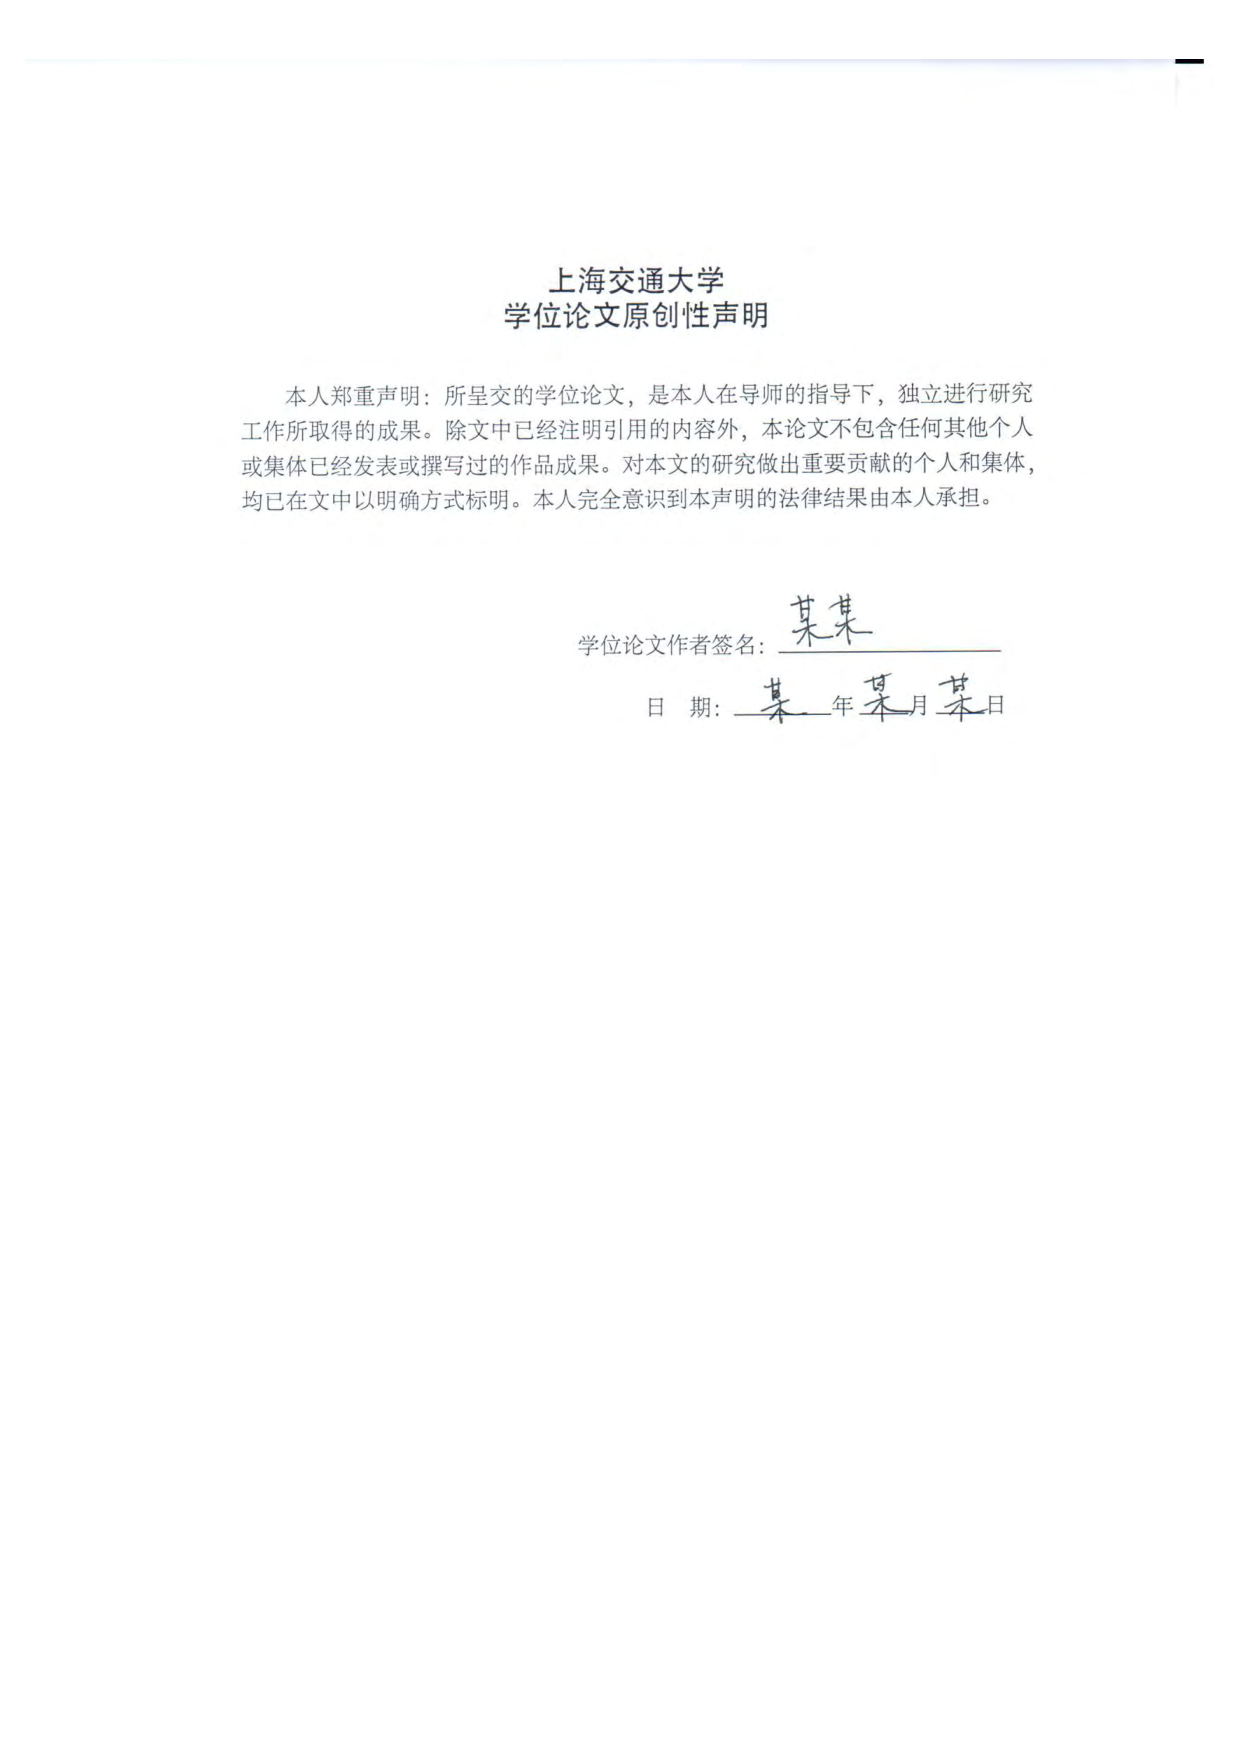
\includepdf{pdf/original.pdf}
	\cleardoublepage
	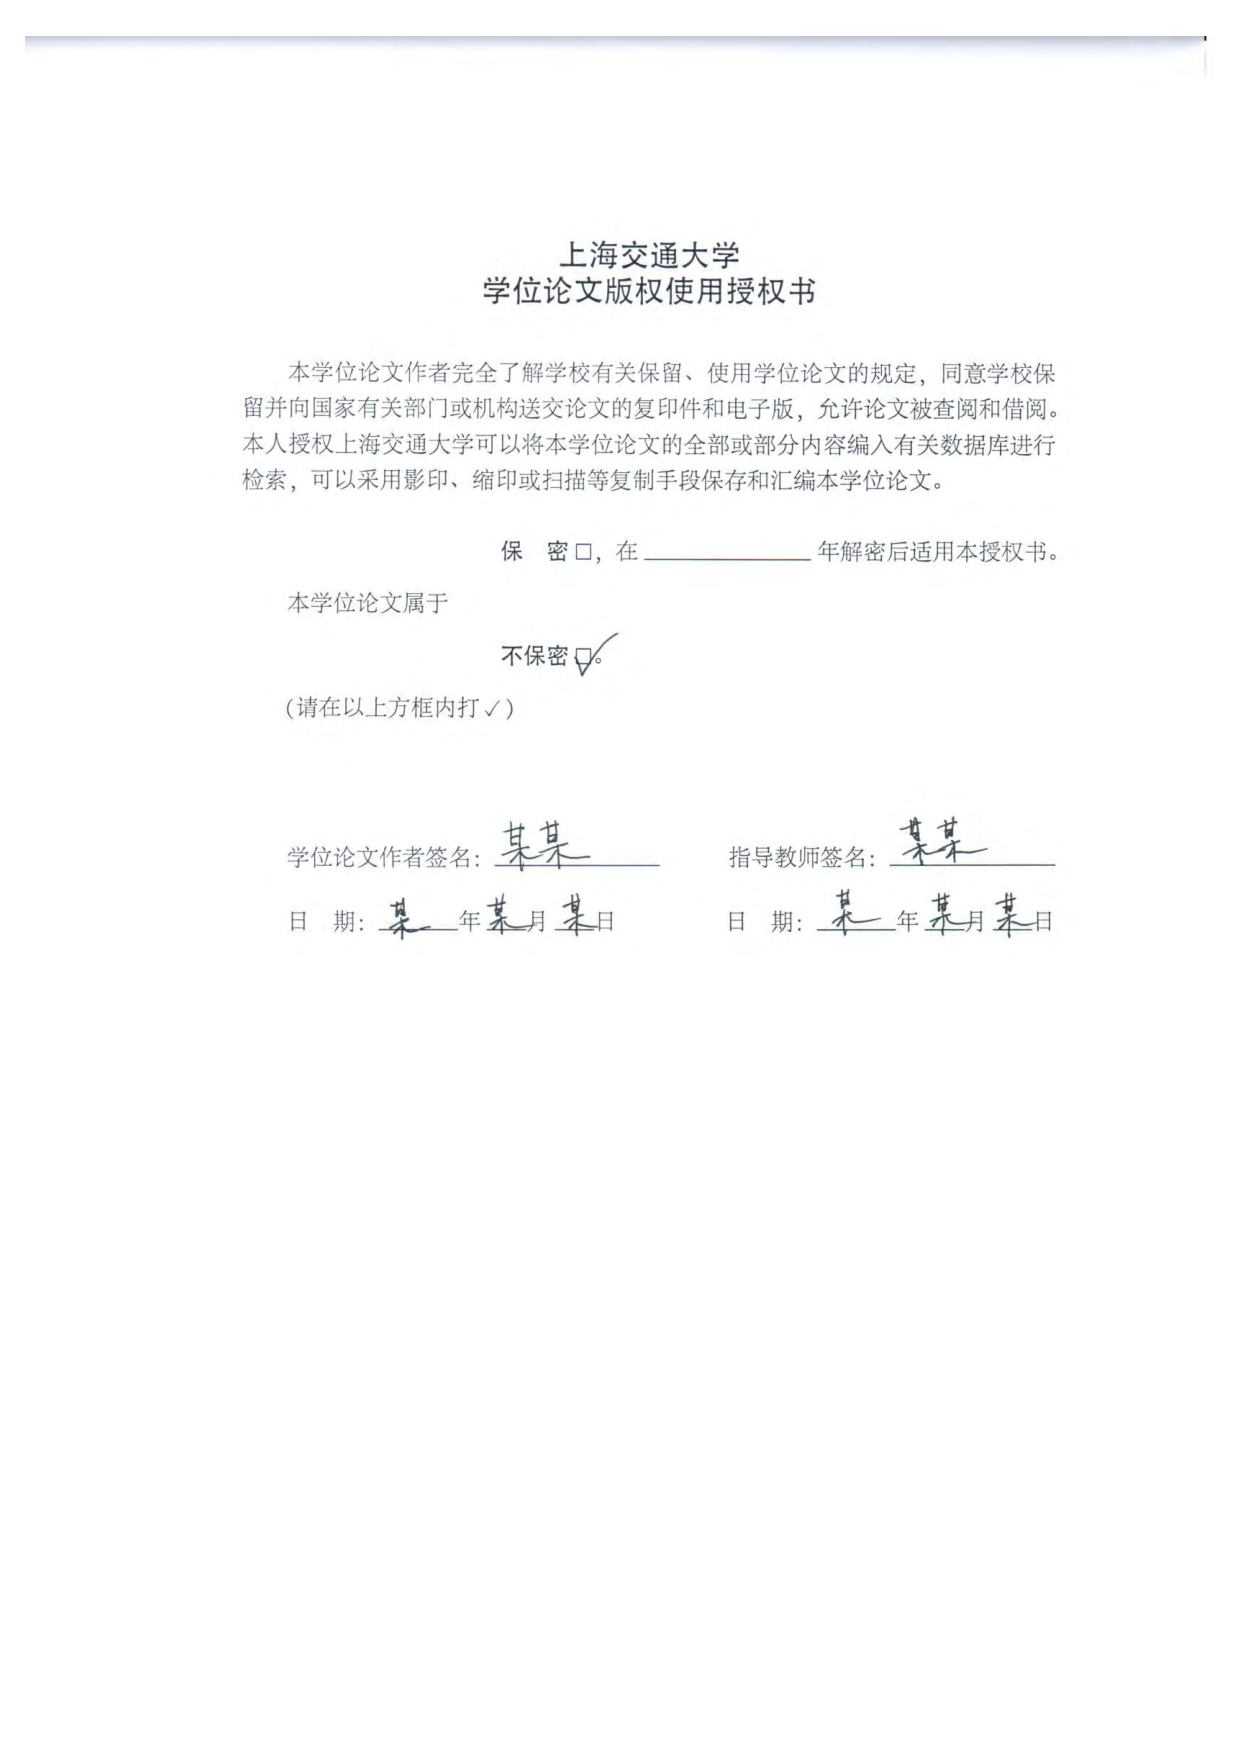
\includepdf{pdf/authorization.pdf}
	\cleardoublepage
\else
	\makeDeclareOriginal
	\makeDeclareAuthorization
\fi
\makeatother


\frontmatter 	% 使用罗马数字对前言编号

%% 摘要
\pagestyle{main}
%# -*- coding: utf-8-unix -*-
%%==================================================
%% abstract.tex for SJTU Master Thesis
%%==================================================

\begin{abstract}
随着分布式电源(Distributed generator, DG)渗透率的不断提高,配电网从传统的无源网络变为有源配电网。大量逆变器接口型分布式电源(Inverter-interfaced DG, IIDG)的接入对电网的安全稳定运行产生日益重要的影响。为了防止电网故障期间IIDG大规模脱网给电网带来严重的不良影响,保证电网的安全稳定运行,并网规程要求,分布式电源在电力系统事故或扰动引起电压跌落时,在一定的电压跌落范围和时间间隔内,能够保证不脱网连续运行,甚至向电网注入额外的无功功率,从而支撑电网电压,实现故障穿越。而且,传统配电网中不对称故障发生的概率最高。因此,为了保证配电网的安全稳定运行,本文提出一种适用于有源配电网的自适应方向保护方案,并在不对称故障的故障穿越运行控制策略下讨论该保护方案具体实现的问题。

相对于高压输电网保护,针对配电网的保护研究还比较薄弱。为此,本文首先对国内外有源配电网保护的发展进行了梳理,并根据有源配电网树状拓扑结构的特征,提出了一种原理简单、经济可靠的继电保护方案,该方案对于不同的故障元件、DG类型以及渗透率、配电网运行模式、配电网重构等都具有自适应性。与差动保护相比,本保护方案具有更优的经济性,适合在主动配电网中大量采用。

接着,为满足并网规程的要求,本文提出一种能够满足并网规程的逆变型分布式电源的故障穿越运行控制策略,建立故障时逆变型分布式电源的等值电路,并在此基础上,研究控制策略的优化方法。通过仿真验证了控制策略和优化方法的有效性。研究结果表明,控制策略有助于提高逆变型分布式电源的故障穿越运行能力,改善故障特性,便于故障分析,为含逆变型分布式电源电网的继电保护原理研究提供参考。与已有研究的主要区别在于,本文提出的控制策略及其故障特征分析方法计及不同的变流器控制策略以及分布式电源的受控电流源特征,能够满足继电保护原理分析以及整定计算需要。

最后,本文讨论了新保护方案关键元件的实现问题,主要研究了方向元件。由于变流器接口型DG提供的短路电流水平较小,其相、序特征皆与传统配电网有较大区别,这使得常规三段式电流保护、方向元件的选择性、速动性、灵敏性得不到保障。另外,配电网中的潮流方向具有很大的随机性。为此,本文分析了传统方向元件在有源配电网中的适应性问题,并提出一种适用于有源配电网的配电网方向元件原理。

本学位论文在中国南方电网有限责任公司科技项目“新型城市配电网自适应保护关键技术研究与试点应用”的支持下完成。

\keywords{\large 有源配电网 \quad 自适应保护 \quad 故障穿越 \quad 控制策略 \quad 故障特征 \quad 方向元件}
\end{abstract}

\begin{englishabstract}

With the continuous increase of the distributed power (DG), the distribution network transforms from the traditional passive network to the active distribution network. A large number of Inverter-Interfaced DG (IIDG) accesses have an increasingly important impact on the safe and stable operation of the power grid. In order to prevent the IIDG large-scale network disconnection during the power grid to bring serious adverse effects to ensure the safe and stable operation of the power grid, grid-connected regulations require that the distributed power supply in the power system accident or disturbance caused by voltage drop in a certain voltage drop Range and time interval, to ensure that no off-line continuous operation, or even to the grid into the additional reactive power, so as to support the grid voltage to achieve fault crossing. Moreover, the traditional distribution network in the probability of the highest asymmetric failure. Therefore, in order to ensure the safe and stable operation of the distribution network, this paper proposes an adaptive directional protection scheme suitable for active distribution networks, and discusses the implementation of the protection scheme under asymmetric fault faulty operation control strategy.

Compared with the protection of high-voltage transmission network, the research on protection of distribution network is still weak. In this paper, firstly, the development of active power distribution network protection at home and abroad is sorted out, and a simple and economical relay protection scheme is proposed according to the characteristics of tree topology of active power distribution network. The scheme is adaptable to different fault components, DG type and permeability, distribution network operation mode, distribution network reconfiguration and so on. Compared with the differential protection, the protection scheme has better economy, suitable for active use in a large number of distribution network.

Then, in order to meet the requirement of grid-connected regulation, this paper proposes a fault-tolerant distributed fault-tolerant distributed power control strategy to establish the equivalent circuit of inverter distributed power supply. Based on this, the optimization method of control strategy is studied. The effectiveness of the control strategy and optimization method is verified by simulation. The research results show that the control strategy can improve the running capability of the fault - tolerant distributed power supply, improve the fault characteristic and facilitate the fault analysis, and provide reference for the relay protection principle of inverter distributed power network. The main difference between the proposed control strategy and the fault feature analysis method is that the different control strategies of the converter and the characteristics of the controlled current source of the distributed power supply can meet the requirements of the relay protection principle analysis and setting calculation need.

Finally, this paper discusses the implementation of the key components of the new protection scheme, and mainly studies the directional components. Because of the short circuit current level provided by converter interface DG, the phase and sequence features are different from the traditional distribution network, which makes the conventional three-stage current protection, directional element selectivity, Sensitivity can not be guaranteed. In addition, the power flow direction in the distribution network is highly random. Therefore, this paper analyzes the adaptability of the traditional directional elements in the active distribution network, and proposes a principle of the directional components of the distribution network which is suitable for the active distribution network.

This dissertation is supported by the "Research and Application of Key Technologies for Adaptive Protection of New Urban Distribution Network", which is a project of China Southern Power Grid Co., Ltd.

\englishkeywords{\large active distribution network,adaptive protection,fault crossing,control strategy,fault feature,direction element}
\end{englishabstract}


%% 目录、插图目录、表格目录
\tableofcontents
\listoffigures
\addcontentsline{toc}{chapter}{\listfigurename} %将插图目录加入全文目录
\listoftables
\addcontentsline{toc}{chapter}{\listtablename}  %将表格目录加入全文目录
\listofalgorithms
\addcontentsline{toc}{chapter}{算法索引}        %将算法目录加入全文目录

%# -*- coding: utf-8-unix -*-
\chapter{主要符号对照表}
\label{chap:symb}

\begin{longtable}{rl}
$\epsilon$     & 介电常数 \\
 $\mu$ 		& 磁导率 \\
 $\epsilon$     & 介电常数 \\
 $\mu$ 		& 磁导率 \\
 $\epsilon$     & 介电常数 \\
 $\mu$ 		& 磁导率 \\
 $\epsilon$ 	& 介电常数 \\
 $\mu$ 		& 磁导率 \\
 $\epsilon$     & 介电常数 \\
 $\mu$ 		& 磁导率 \\
 $\epsilon$     & 介电常数 \\
 $\mu$ 		& 磁导率 \\
 $\epsilon$     & 介电常数 \\
 $\mu$ 		& 磁导率 \\
 $\epsilon$ 	& 介电常数 \\
 $\mu$ 		& 磁导率 \\
 $\epsilon$     & 介电常数 \\
 $\mu$ 		& 磁导率 \\
 $\epsilon$     & 介电常数 \\
 $\mu$ 		& 磁导率 \\
 $\epsilon$     & 介电常数 \\
 $\mu$ 		& 磁导率 \\
 $\epsilon$ 	& 介电常数 \\
 $\mu$ 		& 磁导率 \\
 $\epsilon$     & 介电常数 \\
 $\mu$ 		& 磁导率 \\
 $\epsilon$     & 介电常数 \\
 $\mu$ 		& 磁导率 \\
 $\epsilon$     & 介电常数 \\
 $\mu$ 		& 磁导率 \\
 $\epsilon$ 	& 介电常数 \\
 $\mu$ 		& 磁导率 \\
 $\epsilon$     & 介电常数 \\
 $\mu$ 		& 磁导率 \\
 $\epsilon$     & 介电常数 \\
 $\mu$ 		& 磁导率 \\
 $\epsilon$     & 介电常数 \\
 $\mu$ 		& 磁导率 \\
 $\epsilon$ 	& 介电常数 \\
 $\mu$ 		& 磁导率 \\
 $\epsilon$     & 介电常数 \\
 $\mu$ 		& 磁导率 \\
 $\epsilon$     & 介电常数 \\
 $\mu$ 		& 磁导率 \\
 $\epsilon$     & 介电常数 \\
 $\mu$ 		& 磁导率 \\
 $\epsilon$ 	& 介电常数 \\
 $\mu$ 		& 磁导率 \\
 $\epsilon$     & 介电常数 \\
 $\mu$ 		& 磁导率 \\
 $\epsilon$     & 介电常数 \\
 $\mu$ 		& 磁导率 \\
 $\epsilon$     & 介电常数 \\
 $\mu$ 		& 磁导率 \\
\end{longtable}
 % 主要符号、缩略词对照表

\mainmatter	% 使用阿拉伯数字对正文编号

%% 正文内容
\pagestyle{main}
\chapter{绪论}
\label{chap:introduction}

\section{研究背景及意义}

电力产业是关系到民生国计的基础产业,电力的安全供应关系到国家安全战略,以及经济社会发展。随着化石能源的不断枯竭以及大气污染的日益加剧,优化能源结构、构建清洁低碳、安全高效的现代能源体系成为国家能源战略的重要方向。

近年来,为了提高供电可靠性、降低网损、改善环境以及支持需求侧响应,分布式可再生能源迅速发展,越来越多的分布式电源(Distributed Generation,DG)如分布式光伏、风电、电动汽车、储能装置以及微网开始大量接入配电网。传统的配电网是一个功率单向流动的无源网络,而大量DG的接入对传统配电网的拓扑结构、运行规程、控制方式和保护配置等都提出了很大的挑战。

从继电保护角度,未来的变化趋势以及面临的挑战主要包括以下几个方面:首先是短路电流方向特征的变化。DG接入后,改变了传统配电网中短路电流的单向性;其次是短路电流水平的变化。大多分布式可再生能源属于逆变器接口型DG\cite{ustun2011central,naderi2016efficient}(Inverter-interfaced DG,IIDG),所能提供的短路电流水平有限,一般仅为额定电流的1.2倍。此外,某些主动配电网具备特殊情况下的微网运行能力,其在联网和孤岛运行模式下的短路电流具有很大差异。这些都给保护的整定与配合带来了极大的困难;第三,主动配电网具备故障后重构以及正常运行时的优化重构能力,而网络重构会改变拓扑结构,保护必须能够做到迅速适应;第四,在主动配电网中,母线上有源线路增多,进一步增大了配置专用母线保护的成本;最后,仍需要把经济性作为重要约束条件,在设计保护方案时应充分考虑投资成本和运维成本。

目前应对含DG的配网保护主要措施有:DG在配网故障时立即退出;限制DG在配网中的接入位置和接入容量;在DG支路增加限流器限制DG贡献的故障电流,这些做法虽然不需要改变原有配网保护系统,但一定程度上破坏了DG的正常运行,没有从根本上解决含DG的配网保护问题。尚处于理论研究阶段的保护方案中,采用多代理的智能保护设计依赖的信息较多、判断方式较复杂,距离实际运用较远;改变原有的电流保护方案,引入方向启动判据是一种整体效果较好的解决方案\cite{shangjin2013}。

现有变流器仿真模型以稳态和机电暂态过程仿真为主,不能准确反映故障电流的时域特征,不能适应保护原理的研究;虽然有模型在电力电子器件部分采用了详细模型,但控制策略较为简单,仅考虑了稳态运行时控制的基本要求,未能计及各种控制策略(如正序、负序控制)、及变流器电流限制;导致不能满足并网规程中故障穿越的要求,也无法兼顾不对称故障的情况,不能适应保护原理的研究。为此,有必要针对继电保护的需要,建立变流器接口型分布式电源的通用故障分析模型,形成实用化的短路电流计算方法。

传统的方向元件通过比较故障电流和参考电压的相位来获得故障方向,需要同时安装电流互感器和电压互感器。这对于线路数量庞大的配电网是不可接受的,一方面增设电压互感器的成本过高;另一方面,此类方向元件存在“近区故障”,即当故障点与保护安装处距离过近时,无法判断故障方向。文献\cite{gao2006design}改进了传统方向性保护的灵敏性和可靠性,用比幅替代比相,解决了因测量电压或电流太小而导致无法判断故障方向的问题,但仍然需要安装电压互感器。仅需电流信息的方向元件不仅可以免除安装电压互感器的成本,还能够解决“近区故障”问题\cite{pradhan2008solution}。因此,研究适用于含DG配电网的方向元件很有必要。

国外学者虽然在有关自适应保护相关的讨论进行了很多年,但实际应用依旧较少。文献\cite{laaksonen2014adaptive}在芬兰的Hailuoto Island上实现了一套自适应的保护与微网控制系统,并投入了实际运行。该系统设置了一个中央控制单元,能够实时检测配电网是否运行与并网或孤岛状态,并根据运行状态的不同切换保护定值,从而实现自适应。但该系统所关注的重点(并网/孤岛运行模式的自适应)与本项目(对配电网结构的自适应,对DG投入/退出的自适应,以及提高保护的选择性和速动性等)不同。

我国学者也对自适应保护做了较多研究,并形成了很多重要的理论成果\cite{yaozhong2007}。但是,相关研究主要针对高压输电网保护。由于传统配电网拓扑结构较为单一、保护配置较为简单,针对配电网的自适应保护研究很少,且缺乏工程应用。


\section{有源配电网对保护系统的影响}

\subsection{有源配电网的发展趋势及对保护的挑战}

随着大量分布式电源(Distributed Generator, DG)接入配电网,传统的单向供电的被动式配电网正在向着能够可靠地完成DG 的消纳、调度、保护和监控的主动配电网方向演变\cite{tianming2013,lipeng2009}。在具有高渗透率DG的主动配电网中,配电网的潮流、短路电流特征将产生实质性的改变\cite{zhang2016new,manditereza2016,huang2016diagnostic},继电保护技术将面临多方面挑战。

第一,在传统城市配电网中的保护一般按照闭环运行来设计,但是实际运行时,配电网是开环运行的,这样保护的配置能够简化。但对于高渗透 DG 的智能配电网,故障电流的单向特性不再存在。配电网采用闭环方式运行可以显著提高供电可靠性、确保线路的电压水平,因此,未来的城市配电网应该有闭环运行能力。然而,在传统的配电网三相电流保护没有方向元件或没有电压互感器配置,很难适应上述趋势。

第二,与常规集中式发电不同的是,DG具有容量小、数量多的特点,运行人员不具备对DG单元的直接控制能力,这意味着配电网的电能质量甚至运行的安全性都难以得到保障。为此,应考虑在DG接入配电网的公共耦合点配置一种接口保护,以使DG能够满足相关并网导则,并简化配电网保护与DG自身保护的协调配合。

第三,DG多点接入配电网后,在进行配电网整定计算时,需考虑系统电源以及DG的多种组合运行方式。这无疑极大增加了短路计算的工作量;由于配电网线路一般较短,保护上下级之间很难配合。这样,整定计算变得非常复杂。仅靠定值和时间的配合已难以保证保护的选择性、灵敏性和速动性。而合理引入光纤通信技术,利用通信来保证保护性能并简化整定计算,成为一种重要的技术趋势。而IEC 61850在高压变电站中的大量成功应用,为实施新型城市配电网保护提供了互操作保证。

第四,很多DG(如风、光、储等)以变流器接入配电网,其故障电流水平与传统的同步发电机存在很大差异,其故障特征从传统的电压源变为受控的电流源。为了满足并网导则的要求,在系统发生不对称故障时,变流器会主动向配电网注入负序电流以提高公共耦合点电压的对称性,同时减少输出功率中的二次脉动分量。这使得变流器接口型DG的相、序故障特征发生了很大变化,给以同步电机故障特征为理论基础的传统保护原理带来了很大挑战。

为了应对上述问题,近年来研究者做出了大量努力\cite{ruisheng2015yi,houlei2014,ruisheng2015shi,liukai2014zhu,nikolaidis2016communication,libin2010han,peichao2016zhi}。由于差动保护可以很好地解决输电网络中双向潮流的问题\cite{ruisheng2015yi},文献\cite{houlei2014}把差动保护应用于配电网,采用基于正序故障分量的电流差动保护原理,有效适应配电网线路特点并能够解决弱馈问题。文献\cite{ruisheng2015shi}采用基于配电自动化的集中式线路差动和就地式母线差动的保护方案,能够适用于主动配电网。但差动保护对通道和同步要求很高\cite{liukai2014zhu},投资成本大、运维复杂,在配电网中大量采用具有困难。

\subsection{适用于有源配电网的保护研究目标}

由上可见,随着DG在城市配电网中的高密度接入,将使得城市电网的电源、负荷及供电特征发生重大变化。为了使得城市配电网能够接纳大量DG,应抓紧研究、示范能够适应上述变化的新型有源配电网自适应保护关键技术。相关关键技术研究与示范应达到如下目的:

第一,自适应性。新型保护方案应能适应配电网的辐射型或环型供电拓扑结构;能够适应DG的随机性以及投入/退出等多种运行方式;能够适应配电网中线路、母线等各种故障位置和故障类型,通过自适应能力,实现全线速动。

第二,经济性。采用一体化、多功能保护装置,减少装置数量;避免采用差动保护来保证绝对的选择性,以降低保护部署和运维的成本;研究无需PT的方向元件。

第三,可靠性。保护原理和方案应能减少保护定值、降低保护上下级配合的复杂性,减少因整定配合所导致的保护不正确动作;充分考虑保护拒动、断路器失灵、通信失效等异常情况,并提供完善的后备保护功能

\section{主要内容与技术路线}

本文首先介绍了配电网中分布式发电并网保护的定义和必要性,分析了其应具备的功能及相应的性能要求。由于并网保护功能的多样性和配置的复杂性,提出采用机器学习的方法实现其中的故障检测和孤岛检测功能。通过理论比较分析,本文采用了泛化能力更优的SVM算法,在传统的二分类基础上,经过概率建模构建并网保护的三分类模型,通过仿真实现并与常规的保护性能进行了比较。最后,为了解决智能型保护实际应用中可能存在的概念漂移现象,针对并网保护中的孤岛检测功能,研究了在线自学习的实现方法。本文将通过六个章节对上述内容展开研究,各章内容如下:

第一章:绪论。分析了含有DG的配电网中保护配置和整定所面临的困境,及采用机器学习方法实现保护原理的优势,并从故障保护和防孤岛保护两方面介绍了国内外已提出的智能保护原理,说明了机器学习方法在继电保护领域的研究现状。

第二章:分布式发电并网保护。梳理了国内外对DG并网保护的研究现状;综合多个标准规程,给出了并网保护的定义,并从故障检测、孤岛检测和检同期等方面分析了并网保护应具备的保护功能及基于常规保护的配置方案。然后针对其中的故障检测和孤岛检测功能分析了相应的性能要求。最后,从并网标准和保护原理两方面讨论了以后可能的研究方向。

第三章:机器学习基本理论与方法。针对并网保护配置复杂、整定困难等问题,本文提出了基于机器学习的解决思路。为此,本章专门对机器学习方法及常用的分类算法作了介绍。通过分析SVM算法的基本理论,比较得出了其理论上的优势,因此确定了本文采用的基本分类算法。最后说明了基于机器学习的智能保护原理的特有优势及目前还待解决的一些问题。

第四章:基于多分类支持向量机的分布式发电并网保护。为了同时实现DG并网保护中的故障检测和孤岛检测功能,本章在传统二分类SVM的基础上进行改进,通过概率建模的方法构建三分类模型,同时能够给出预测类别的概率估计。采用了SVM-RFE特征选择算法结合交叉验证,以提高分类模型的泛化能力。最后,通过对变流器接口型DG和同步电机型DG并网保护的算例进行仿真证明了该方案比常规保护性能上更加可靠。

第五章:主动配电网中基于在线自学习的孤岛检测方法。针对主动配电网中在线孤岛检测时易出现的概念漂移现象,本章提出了在线聚类抽样和优选样本集相结合的在线学习方法。另外,针对实际电网运行样本中孤岛类样本远远少于非孤岛类样本,而导致样本集类别分布不均衡的问题,本章采用了加权SVM算法结合新的评价指标以减弱非均衡数据集的影响。最后通过仿真分别测试了在线聚类抽样和优选样本集策略,证明了所提方案的可行性和合理性。

第六章:总结全文,介绍本文取得的工作成果和课题后续展望。

\chapter{级联闭锁自适应方向保护原理}

为了对各种配电网结构都具有适应性,能支持支持开环和闭环多种运行方式,能适应配电网工作于孤岛、并网两种模式,本章研究基于自适应级联方向闭锁原理的配电网电流保护方案;采用本方案后,无需额外配置专门的母线保护,能够快速切除母线故障,避免扩大停电范围。与差动保护相比,本保护方案具有更优的经济性,适合在主动配电网中大量采用。

\section{有源配电网保护研究的发展}

如第一章所述,传统的配电网保护难以适应配电网的新变化。为此,国内外诸多学者提出了多种新型保护方案。可以根据保护方案是否需要依赖通信,把这些新型配电网保护方案分成两大类。

第一类保护方案只需要本地的信息。由于不依赖通信,故在可靠性与成本方面有明显优势。

文献\cite{ganzhong2002shu}提出一种基于突变量和系统不平衡度的保护方案,只需要线路一侧的电气量,不需要通讯通道,然而这种保护方案的整定难度很大,而且不能用于对称故障的情况。
文献\cite{zamani2011protection,najy2013optimal,hsieh2014adaptive,zeineldin2015optimal}提出了能够用于有源配电网的电流方向保护方案,但是
文献\cite{najy2013optimal}的方案需要使用限流器,而且只对应用于同步机型分布式电源的场景做了具体分析;
文献\cite{zamani2011protection}的方案通过保护限时的层层配合来保证选择性,这样故障切除的时间会很长,而且该方案只能用在工作在开环方式下的配电网。
文献\cite{dewadasa2010fold}把导纳作为特征量,形成反时限保护方案,文献\cite{wentao2014wei}提出了利用低阻抗特性实现保护方案,但是由于配电网的线路比较短,因此这两种方法应用于配电网时其整定值很难互相配合。
文献\cite{hsieh2014adaptive,zeineldin2015optimal}采用反时限过电流保护的逐级配合原理,同样这种方案的总体动作速度很慢,另外实现复杂度很高。
综合以上文献结果可以看出,这类不依赖通信的保护方案的速动性和易实现性有所不足。

第二类保护方案需要靠通信技术传输信息。根据所通信信息的类型,又可以分为两种。一种需要通信模拟量的信息,比如数字式的差动保护\cite{qing2014recent}。但这种方法需要传输的信息量极大,需要解决克服大量信息实时通信特有的问题,比如同步问题、带宽问题等等,离实际应用还有相当大的距离。另一类仅需交换逻辑量的信息,比如故障方向的判断结论。由于传输的信息量不大,对通信带宽要求低,而且不需要同步采样,这种方案更有希望实际应用于有源配电网。文献\cite{wangwei2009}提出了区域纵联方向保护方案,采用一主多从的系统架构。但在这个方案中,一旦保护主机发生故障,整个保护系统都不能正常运行。

\subsection{级联闭锁电流保护方案}

在不含DG的辐射型配电网中,如图\ref{fig:interlocking}所示的级联闭锁保护方案早已被采用\cite{yong1990optimizing},闭锁信号利用屏蔽双绞线级联传输,闭锁方向固定由负荷侧指向电源侧(系统侧)。设F点发生故障,则保护PR4~PR1的过电流保护都起动并向上游保护发送闭锁信号。保护PR5因感受不到故障电流而不发闭锁信号。最终,保护PR4因收不到闭锁信号而动作切除故障。可见,该方案对于传统辐射型配电网具有明确的选择性。

\begin{figure}[!htp]
  \centering
  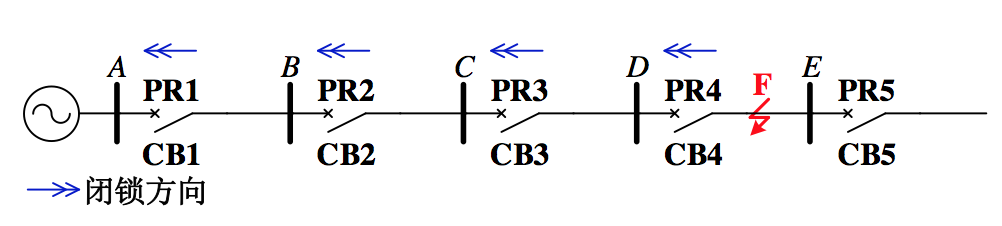
\includegraphics[width=0.6\textwidth]{chap2/interlocking}
  \bicaption[fig:interlocking]{级联闭锁电流保护方案}{级联闭锁电流保护方案}{Fig.}{Interlocking overcurrent protection schema}
\end{figure}

上述级联闭锁方案中不配置方向元件,因而当配电网含有DG或采用闭环拓扑时将失去选择性。为此,文献\cite{libin2010han}提出为电流保护增加方向元件,构成适合闭环配电网的级联方向闭锁纵联电流保护方案。例如在图\ref{fig:interlocking}中,在为电流保护增加方向元件后,在具有相同参考方向的一组保护中,如PR1~PR5,就可以继续采用上述级联闭锁方案。但该方案不具备母线保护功能,母线故障需要依靠相邻变电站切除。例如,变电站D的母线故障需要变电站C、E的保护动作切除。

\subsection{级联方向闭锁电流保护方案}

对于环型供电网络,或者接入了DG的辐射型配电网,文献\cite{oudalov2009adaptive}提出了另外一种针对含DG配电网的级联方向闭锁保护方案,在受影响的保护处增加方向元件,从而将保护分为两组,如图\ref{fig:directional}所示。与文献\cite{libin2010han}采用固定闭锁方向所不同的是,其闭锁方向会随着故障点的不同而自适应改变,克服了上一方案的缺点。但该文提出的方案同样不具备母线保护功能,且不能适应闭环配电网。但本方案不具备母线保护功能,母线故障需要依靠相邻变电站切除。例如,变电站D的母线故障需要变电站C、E的保护动作切除。另外,该文对所提出的保护方案缺乏具体实现方案和分析验证。

\begin{figure}[!htp]
  \centering
  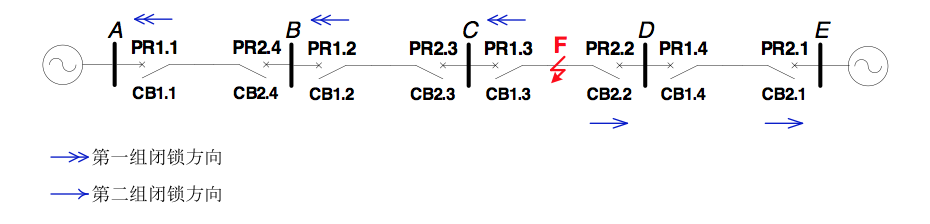
\includegraphics[width=0.6\textwidth]{chap2/directional}
  \bicaption[fig:directional]{级联方向闭锁电流保护方案}{级联方向闭锁电流保护方案}{Fig.}{Directional interlocking overcurrent protection schema}
\end{figure}

方向闭锁原理能够实现线路故障的全线速动,同时无需同步采样且对通信带宽要求低,故较之差动保护具有更好的经济性。文献\cite{liukai2014zhu,nikolaidis2016communication,libin2010han}提出了几种方向闭锁纵联电流保护方案,其中,文献\cite{liukai2014zhu,nikolaidis2016communication}针对辐射形配电网,而文献\cite{libin2010han}则适合闭环运行配电网。但这些方案仅具备线路保护功能,而在配电网中,母线故障概率较高,且易造成开关设备烧毁,甚至烧坏直流操作回路造成整站保护拒动。但中低压母线一般不设专门的母线保护,母线故障需靠相邻线路保护切除,动作时间较长,并且往往要扩大停电范围。

在以上原理的基础上,本文提出的自适应级联方向闭锁电流保护方案同时具备快速线路和母线保护功能,且能适应开环和闭环等多种配电网结构。

\section{面向环形配电网的自适应方向保护方案}

\subsection{方向闭锁保护原理}

图\ref{fig:schematic}为本保护方案的原理示意图,图中每套保护(Protective Relay,PR)由方向元件和启动元件组成。

\begin{figure}
    \centering
    \subfigure[配电网正常运行]{
        \begin{minipage}[b]{0.5\textwidth}
        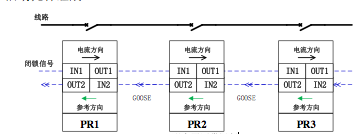
\includegraphics[width=1\textwidth]{chap2/schematic_a}
        \label{fig:schematic_a}
        \end{minipage}
    }
    \subfigure[故障后新的闭锁方向]{
        \begin{minipage}[b]{0.5\textwidth}
        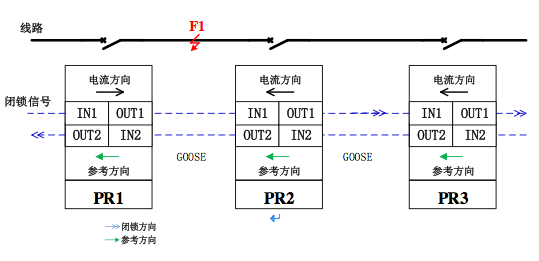
\includegraphics[width=1\textwidth]{chap2/schematic_b}
        \label{fig:schematic_b}
        \end{minipage}
    }
    \bicaption[fig:schematic]{自适应方向保护原理示意图}{自适应方向保护原理示意图}{Fig.}{Schematic of adaptive directional protection}
\end{figure}

保护的参考方向设置为$PR3 \to PR2 \to PR1$,如图\ref{fig:schematic} \subref{fig:schematic_a}。当F1处发生故障时,PR1、PR2、PR3的过流元件皆起动,PR1判别出故障方向异于参考方向,而PR2、PR3的故障方向同于参考方向,如图\ref{fig:schematic} \subref{fig:schematic_b}。为正确切除故障,PR1需要顺着参考方向发送闭锁信号,而PR2、PR3则需逆参考方向发送闭锁信号。这样,F1处故障才可以被保护PR1、PR2选择性切除,而其余保护则被闭锁。

原理的保护跳闸条件为本地过流保护起动,并且未收到闭锁信号。判据如下:

\begin{equation}
    \label{eq:trip}
    Trip = NOT (BlockingSignal) AND (I>I\_set) 
\end{equation}}
	 
式\ref{eq:trip}中,$BlockingSignal$指收到的闭锁信号,$I\_set$为本地过流保护起动定值,按躲最大负荷整定。

利用GOOSE交换闭锁信号,可以大量减少控制电缆,提高保护之间的互操作性。同时,还可以充分利用GOOSE的通信自检机制,提高保护的可靠性。根据GOOSE的收发原理,在图2中,每套保护设置了两组、四个GOOSE虚端子。其中,第一组虚端子IN1、OUT1负责逆参考方向闭锁信号的接收与发送;第二组虚端子IN2、OUT2则负责顺参考方向闭锁信号的收发。在智能配电网中,可以根据不同需要,选择光纤、电力线甚至无线网络等多种介质\cite{huangfei2013ji,parikh2013comprehensive,kanabar2009evaluation}完成GOOSE的收发。

\subsection{参考方向和闭锁方向规则}

由上可见,为了保证自适应方向保护方案的选择性,需要建立参考方向和闭锁方向的相关规则。

以图\ref{fig:cankao}所示的典型环型和辐射型配电网为例,本文定义如下参考方向的整定规则:

\begin{figure}
    \centering
    \subfigure[环型配电网]{
        \begin{minipage}[b]{0.5\textwidth}
        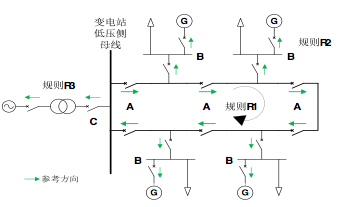
\includegraphics[width=1\textwidth]{chap2/cankao_a}
        \label{fig:cankao_a}
        \end{minipage}
    }
    \subfigure[环型配电网]{
        \begin{minipage}[b]{0.5\textwidth}
        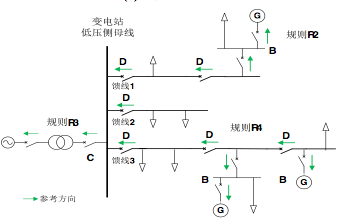
\includegraphics[width=1\textwidth]{chap2/cankao_b}
        \label{fig:cankao_b}
        \end{minipage}
    }
    \bicaption[fig:cankao]{参考方向整定规则示意图}{参考方向整定规则示意图}{Fig.}{Schematic of rules of reference directions}
\end{figure}

\textbf{R1}:环网中馈线断路器(图\ref{fig:cankao}中A所示)的参考方向为沿环同向,即同沿顺时针或逆时针方向;

\textbf{R2}:分支线断路器(图\ref{fig:cankao}中B所示)的参考方向为远离主电网方向;

\textbf{R3}:配电变电站断路器(图\ref{fig:cankao}中C所示)的参考方向为指向主电网方向;

\textbf{R4}:辐射型馈线断路器(图\ref{fig:cankao}中D所示)的参考方向为指向主电网方向。

此外,本文定义了如下闭锁方向规则:

\textbf{B1}:若故障电流与参考方向同向,则闭锁方向与参考方向反向。闭锁信号由IN1、OUT1收发;

\textbf{B2}:否则,则闭锁方向与参考方向同向。闭锁信号由IN2、OUT2收发。

上述规则可以用两种基本故障类型加以解释,如图\ref{fig:two}所示。当发生线路故障时,全系统只有F1点呈现图\ref{fig:two} \subref{fig:two_a}所示的汇流特征,导致只有F1点两侧的保护闭锁方向相背,最终仅保护PR1、PR2因收不到闭锁信号而动作,线路故障F1被选择性切除;当发生母线故障时,全系统只有F2点呈现图\ref{fig:two} \subref{fig:two_b}的汇流特征,最终只有保护PR1~PR3因收不到闭锁信号而动作,母线故障F2被选择性切除。

\begin{figure}
    \centering
    \subfigure[线路故障]{
        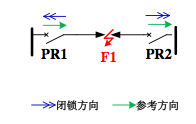
\includegraphics[width=0.3\textwidth]{chap2/two_a}
        \label{fig:two_a}
    }
    \hspace{1in}
    \subfigure[母线故障]{
        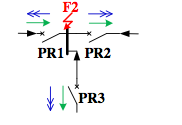
\includegraphics[width=0.3\textwidth]{chap2/two_b}
        \label{fig:two_b}
    }
    \bicaption[fig:two]{两种基本故障类型}{两种基本故障类型}{Fig.}{Two primary fault types}
\end{figure}


\subsection{保护的功能逻辑图}

自适应方向保护方案的实现逻辑如图\ref{fig:logic}所示。

\begin{figure}[!htp]
  \centering
  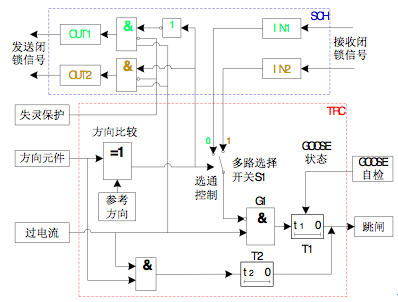
\includegraphics[width=0.6\textwidth]{chap2/logic}
  \bicaption[fig:logic]{自适应方向保护方案的逻辑图}{自适应方向保护方案的逻辑图}{Fig.}{Logic diagram of adaptive directional protection}
\end{figure}

SCH功能块(图中上部虚线框内)实现方向闭锁信号的收发功能。IN1/2、OUT1/2分别对应于图2中保护的两组GOOSE虚端子。

TRC功能块(图中下部虚线框内)根据式(1)实现跳闸条件综合判别功能。首先由方向元件判别故障方向,然后由方向比较模块将其与参考方向比较。如果同向则执行规则B1,此时方向比较模块输出0,控制多路选择开关S1选通端子IN1,并经反相器向OUT1输出闭锁信号;如果反向则执行规则B2,此时方向比较模块输出1,开关S1选通IN2,并向OUT2输出闭锁信号。考虑到闭锁信号的延时,以及相邻保护的起动和返回时间的不一致性,增加了延时动作元件T1。考虑到GOOSE发送延时应小于3ms\cite{baigent2004iec},以及配电网线路较短等因素,延时时间t1可整定为20~100ms。

对于闭锁原理,如果通信失效后发生区外故障,保护会因收不到闭锁信号而误动\cite{shengshi1981}。为解决这个问题,在图5中,利用GOOSE的自检机制,可在1s左右探测到通信失效,并自动增大t1定值(如增大至0.6s)以防止保护误动,同时发送告警信号。当外部故障被切除后,本保护瞬时返回。

如果区内故障但断路器失灵,失灵元件动作并输出1,经反相后闭锁OUT1、OUT2的输出。这样,沿闭锁方向的上一级保护因收不到闭锁信号而以近后备或远后备方式动作并切除故障。

如果下游保护拒动,本方案利用图\ref{fig:logic}中的时间元件T2提供后备保护回路。T2串联在过流元件之后,其时间定值以解环点按照逐级配合原则整定,以传统的定时限过电流方式提供可靠的后备功能。

\subsection{环型配电网中保护动作情况分析}

上节提出一种自适应方向保护方案。该方案同时具备线路和母线保护功能,能够实现配电网全范围故障的快速动作。但从保护可靠性角度,上述方案依旧存在两点不足:

\begin{enumerate}
    \item 当配电网开环运行时,故障点下游保护的短路电流仅由DG提供,属于弱溃系统,其起动元件和方向元件的灵敏度不足;
    \item 电流保护作为起动元件,按躲开最大负荷考虑,配电网故障时,非故障线路的保护仅靠方向元件闭锁,对方向元件的依赖很大,存在误动的可能性。
\end{enumerate}

而且该方案主要针对闭环运行的配电网,而目前配电网仍主要采用开环运行的方式。此外,该文献对配电网重构讨论不足。

本文在上一节的基础上,针对更具代表性的开环运行的主动配电网,根据其树状拓扑结构特点,提出一种原理简单的继电保护方案进一步做出两点改善:

\begin{enumerate}
    \item 线路一侧保护动作时,同时向对侧保护发出联跳信号,从而解决对侧弱溃问题;
    \item 电流保护采用两段配置。其中,\uppercase\expandafter{\romannumeral1}段保护范围为本线路全长,为主电流保护;\uppercase\expandafter{\romannumeral2}段保护范围为相邻线路全长,为后备电流保护。
\end{enumerate}

这样,当配电网发生故障时,仅故障点相邻线路的电流保护会起动,有效减少对方向元件正确性的依赖。该方案具备对短路电流水平的适应性、对拓扑结构改变的适应性以及对不同故障元件的适应性。本方案的原理如图5-4所示。


\section{面向辐射形配电网的改进型保护方案}

\section{本章小结}
\chapter{基于LTE的人群密度预测算法}
\label{chap:algorithm}

基于第二章提到的理论知识,本章节我们将针对基于LTE的人群密度监控算法进行详细的讨论。

根据第二章的理论,我们可以得到一下结论:

\begin{enumerate}
    \item 基于LTE的定位技术对于67\%的用户设备定位精度可以达到40m,并且响应时间能够控制在1s以内。
    \item 使用E-CellID技术和OTDOA技术无需用户安装第三方软件,即可实现在用户移动的过程之中进行定位。
    \item 使用LTE技术定位,在不混合GPS定位技术的前提之下,周围环境对定位精度影响较小。适用于人口密度较大的特大城市的场景。
\end{enumerate}
通过上述的结论,我们通过LTE可以方便的收集用户的定位数据,但是定位精度有限。在本章节的第一部分中我们将会详细的介绍位置特征的收集方式。

在收集到用户设备的位置信息后,我们会分别使单拟合、使用相邻区域特征的GBDT算法和自动编码器提取特征的GBDT算法等算法进行预测。简单的线性拟合算法是通过拟合某个小区内人群总数的变化,通过趋势来预测未来的人口数量。我们分别使用相邻区域人群个数和相邻区域信息熵两种特征加入到GBDT算法当中,分别对各个小区的人口趋势进行预测,最后我们对这两种算法进行对比,分析各自的优劣。

通过上述分析,人群密度预测算法的过程如下。

对于拟合算法犹如下流程:
\begin{enumerate}
    \item 通过收集基站数据,收集用户设备的位置信息。
    \item 通过收集到的用户设备位置信息,计算每个小区的人群密度
    \item 分别对每个小区内的人群密度进行拟合,通过拟合方程预测未来每个小区的人群密度。
\end{enumerate}

对于GBDT预测算法流程如下:
\begin{enumerate}
    \item 收集用户设备的位置信息。
    \item 计算每个小区内的人群密度。
    \item 根据相邻小区和小区内的人群密度抽取特征。
    \item 将得到的特征使用GBDT机器学习模型进行训练。
    \item 使用得到的训练模型对未来的人群密度进行预测。
\end{enumerate}
算法的流程图,如图\ref{fig:algo-flow}所示。

\begin{figure}[!htp]
    \centering
    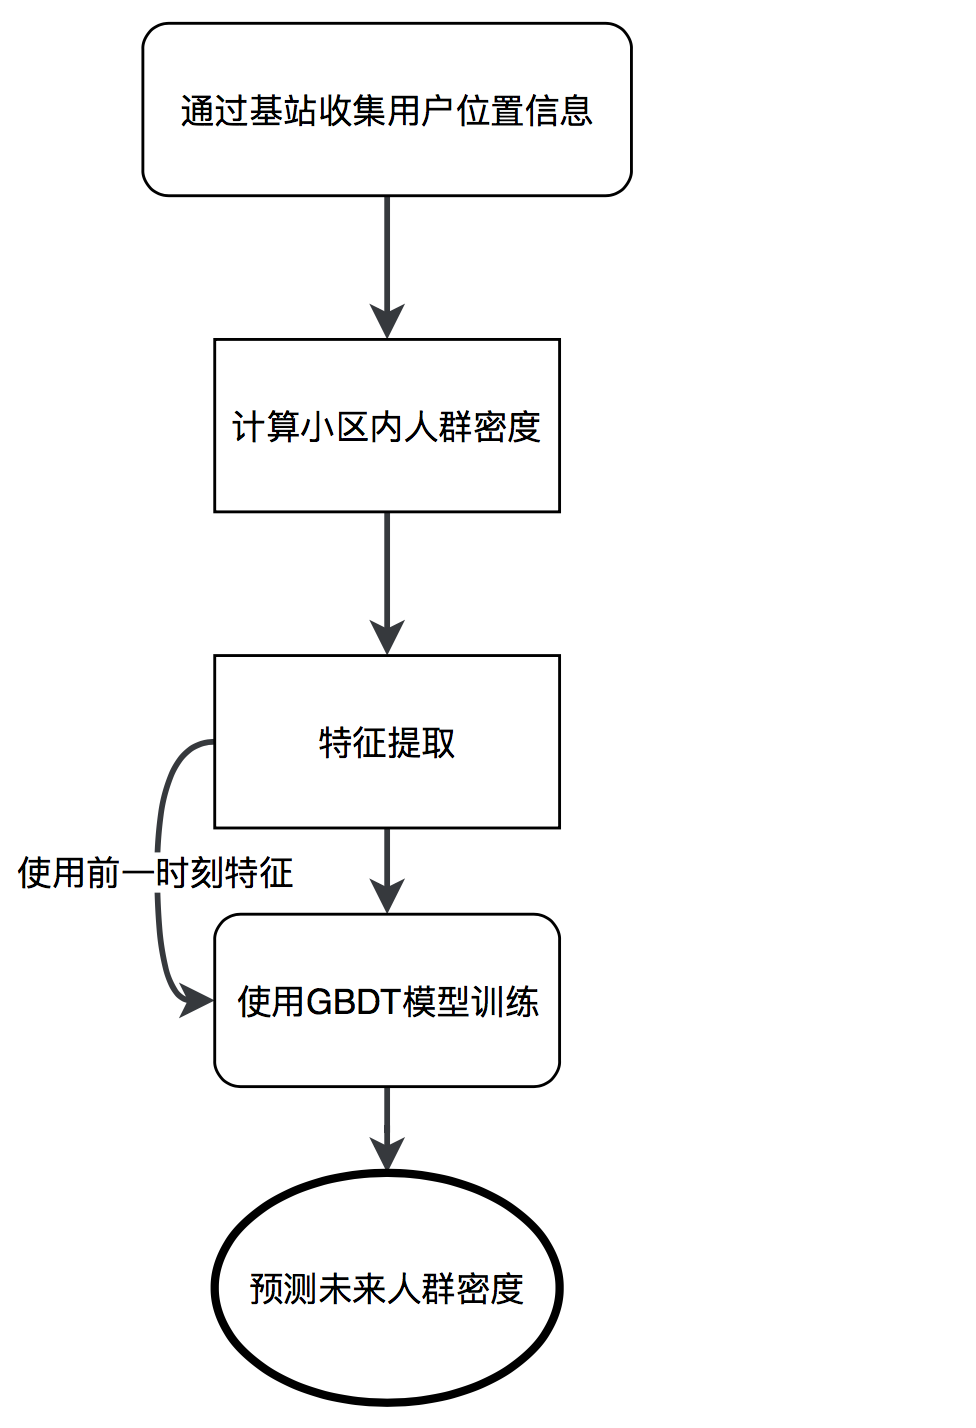
\includegraphics[width=0.8\textwidth]{chap3/algo-flow}
    \bicaption[fig:algo-flow]{算法流程图}{算法流程图}{Fig.}{Algorithm Flowchart}
\end{figure}

\section{位置特征收集}

在当下基于LTE的定位协议经过多年的发展已经逐步稳定,已经能够充分满足定位精度和响应时间的需求。两种新的协议已经被标准化来实现LTE定位:LTE定位协议(英文:Long-term evolution Positioning Protocol,缩写:LPP)\cite{lpp}和LTE定位协议附件(英文:Long-term evolution Positioning Protocol Annex,缩写:LPPa)\cite{lppa}。 LPP是定位服务服务器和定位服务目标设备之间的点对点协议,用于定位目标设备。两个协议中已经规定了以下事务:传输数据,辅助数据传送过程和位置信息传送过程。可以串联或并联使用任何上述类型的多个LPP过程。 LTE定位系统的方框图如\ref{fig:ran-sys}所示:

\begin{figure}[!htp]
    \centering
    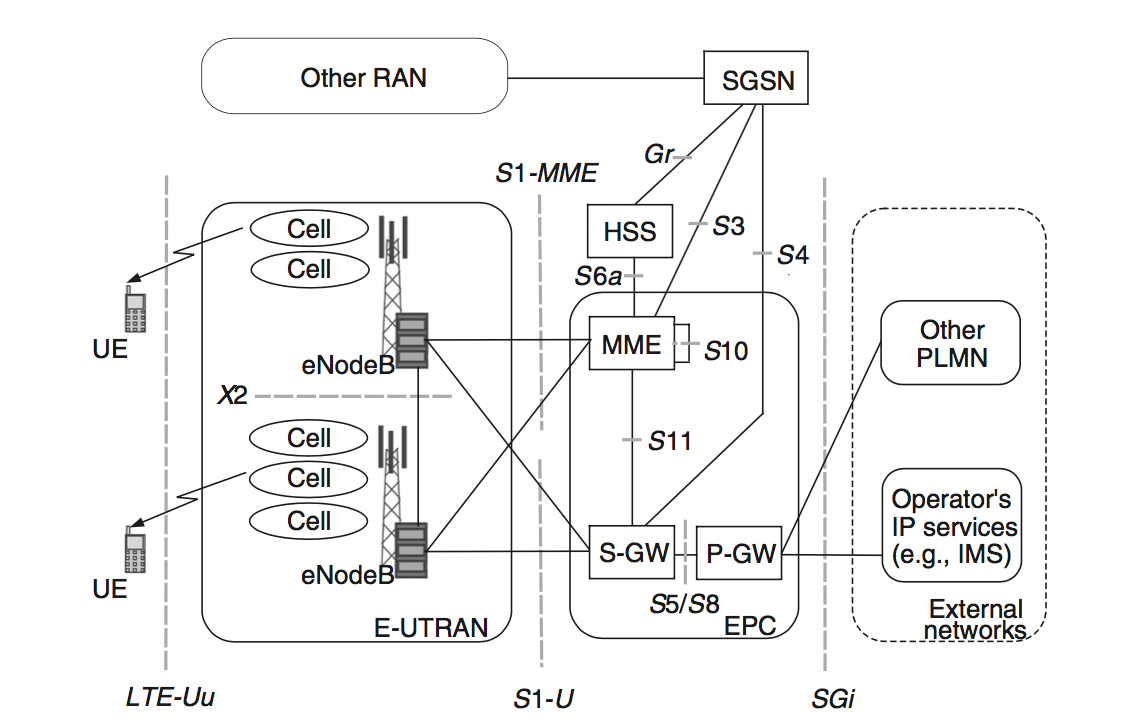
\includegraphics[width=0.8\textwidth]{chap3/ran-sys}
    \bicaption[fig:ran-sys]{LTE系统框架}{LTE系统框架}{Fig.}{LTE System Architecture}
\end{figure}
其中每个\textit{cell}是在LTE系统中含有ID的最小实体,例如Cell ID、用户设备等。每个eNodeB和每个\textit{cell}含有全局唯一的ID,每个eNodeB可以服务多个cell。E-UTRAN与UE之通过在LTE-Uu接口进行无线电通信。在E-UTRAN中,eNodeB可以通过逻辑X2接口互连,逻辑X2接口主要用于移动性和一些无线电资源管理,E-UTRAN通过逻辑接口S1连接到EPC。LTE E-UTRAN接口和协议结构被组织成两个逻辑独立的plane:\textbf{control plane}和\textbf{user plane}。control plane主要用于应用协议,在涉及不同网络节点的若干接口上操作(例如,S1-AP\cite{s1ap}是通过S1接口发送的应用协议,而X2-AP\cite{x2ap}是通过X2接口发送的),以及用于传输也就是传递应用协议消息的信令。其中control plane中的顶层协议是在用户设备和EPC之间操作的非接入层(英文:nonaccess stratum,缩写:NAS)。它使用LTE-Uu接口上的无线资源控制(英文:radio resource control,缩写:RRC)协议和S1接口上的S1-AP协议作为传输协议,而user plane包括由用户平面隧道协议和传输的数据流构成。

对于Control Plane为了支持定位服务(LCS),control plane架构中必须存在至少两个功能节点:演进服务移动定位中心(英文:Evolved Serving Mobile Location Center,缩写:E-SMLC)用于控制定位移动设备所需的资源的协调和调度,以及移动网关定位中心(英文:Gateway Mobile Location Center,缩写:GMLC)用于控制位置数据的传递、用户授权、收费等。使用LTE定位协议进行用于定位相关信息传输。 LPP对移动管理实体(英文:Mobility Management Entity,缩写:MME)也是可见的,然后在使用LPPa在S1-MME和SLs接口上透传数据。control plane的LTE定位架构如图\ref{fig:cp}所示。其中MME接收到与特定LCS目标(例如用户设备)相关联的一些LCS的定位请求。然后,MME在LCS-AP位置请求消息中向LCS发送LCS请求。 E-SMLC处理LCS请求以执行目标用户设备的定位任务。E-SMLC然后将LCS的结果返回给MME。最终MME会将结果转发到请求节点。
\begin{figure}[!htp]
    \centering
    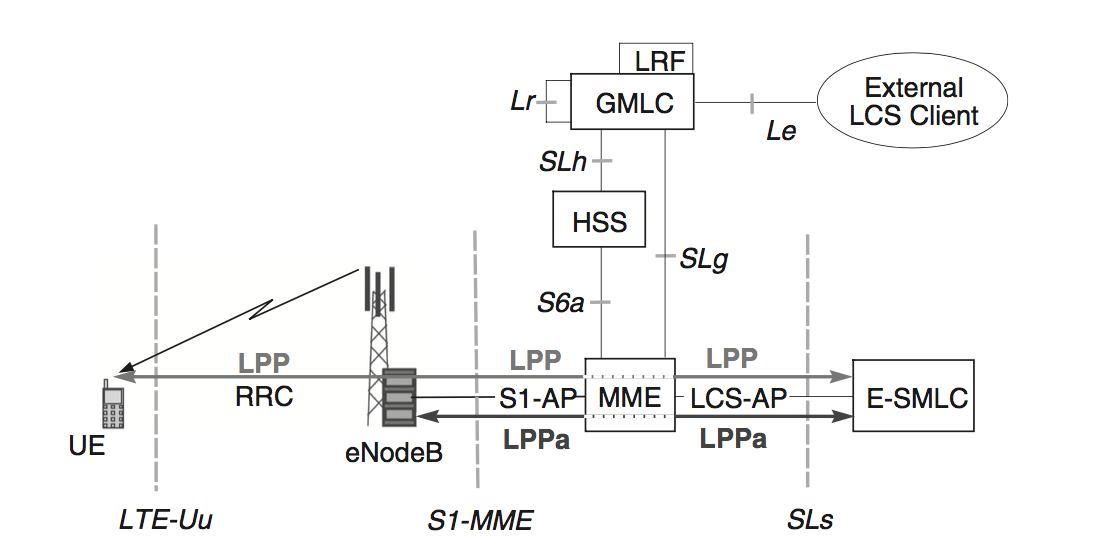
\includegraphics[width=0.8\textwidth]{chap3/control-plane}
    \bicaption[fig:cp]{Control Plane定位框架}{Control Plane定位框架}{Fig.}{Control Plane System Architecture}
\end{figure}

在收到这些信号并通过坐标变换之后,即可通过第二章中提到的定位技术对用户设备进行定位。在LTE定位规范中规定67 \%的设备精度要达到50m,而实际情况中定位精度与用户的信号强度、有无遮挡物、定位服务器负载有着很强的关系。

\section{数据处理}

由于LTE定位精度限制,我们不能将每个行人的精确位置带入到模型当中,我们只能得到行人的大致位置。于是在本文中将采取以下做法,将整个地图区域$A$按照50m为一个单位进行分解,也就是将地图分成网格状结构,于是对于任意一个行人$P_{i}$都可以根据定位得到的坐标$(x, y)$将其放置在地图上的某个方格$A_{m,n}$内。但是我们得到的行人位置并非正确的行人坐标(有着50m左右的误差),于是我们以采集到的行人$P_{i}$的坐标为圆心以25m为半径在地图上画圆,如图\ref{fig:circle}所示,那么我们可以通过每个方格内圆形覆盖的面积得到该行人$P_{i}$在四个方格内的概率,即我们将圆形在方格$A_{m,n}$内覆盖的面积$S_{i,m,n}$作为该行人在区域内的概率,在该时刻对于行人$P_{i}$在方格$A_{m,n}$有$S_{i,m,n}$个人,对地图上所有的人进行上述操作,我们可以得到每个区域中的行人个数,如式\ref{eq:pd}。

\begin{figure}[!htp]
    \centering
    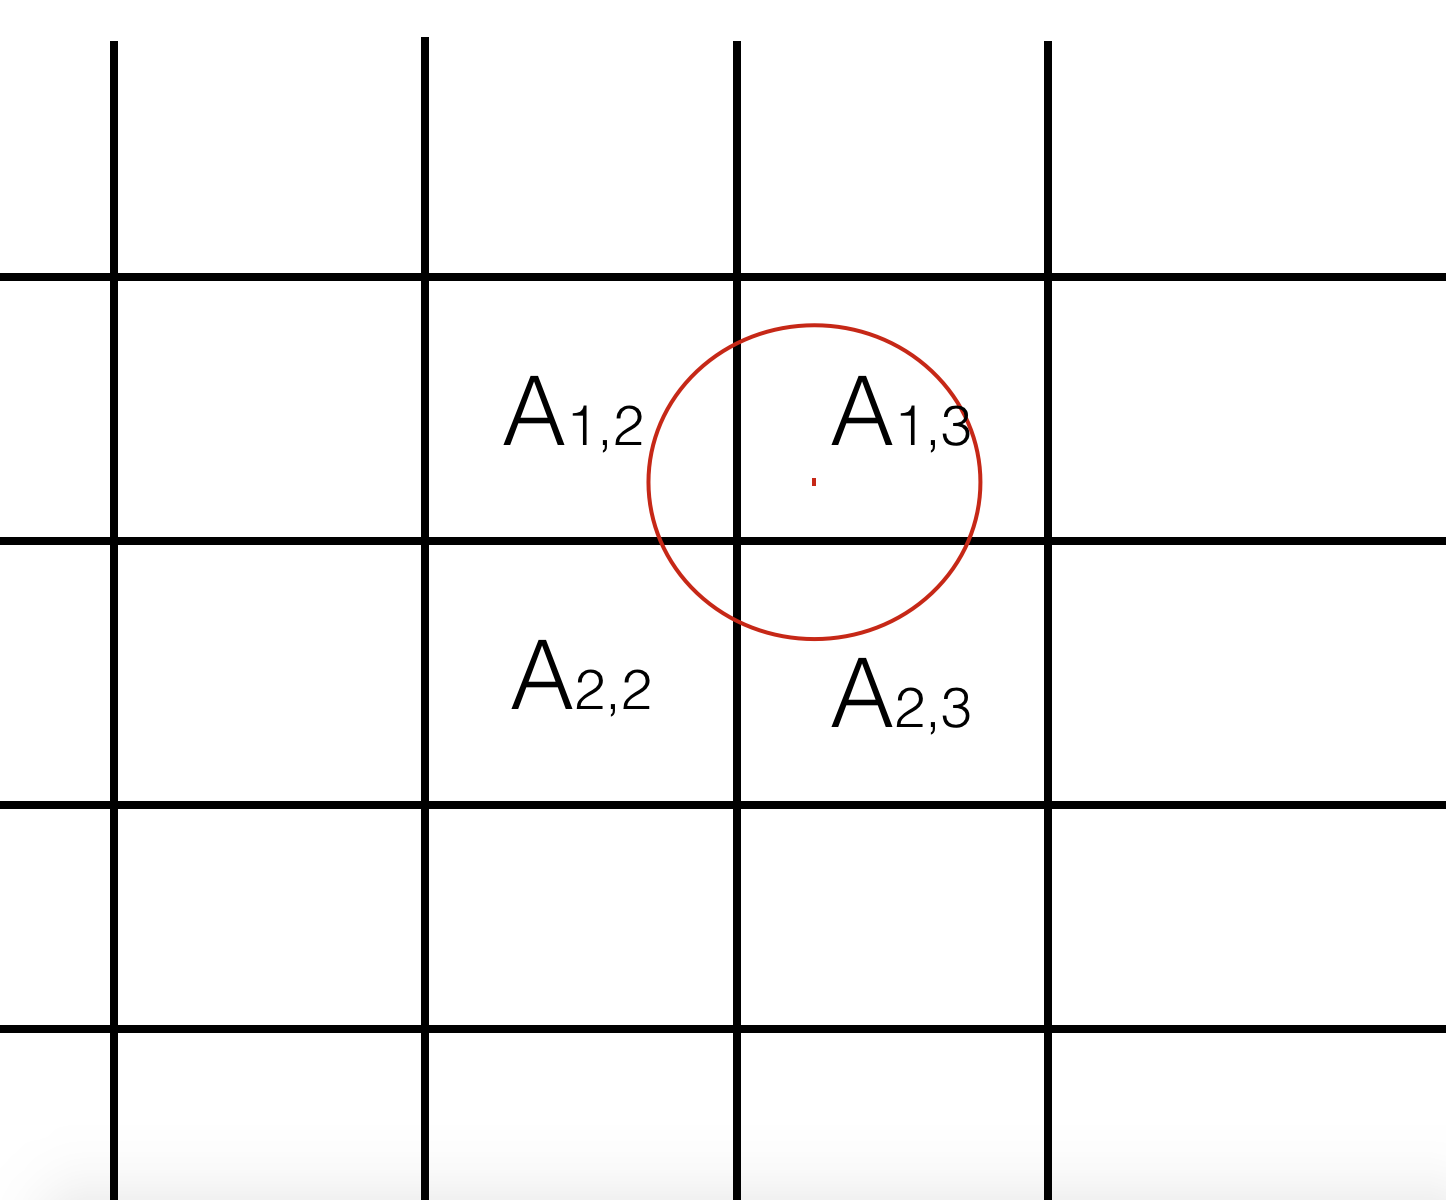
\includegraphics[width=0.6\textwidth]{chap3/circle}
    \bicaption[fig:circle]{行人在区域中分布}{行人在区域中分布}{Fig.}{Pedestrians Circle}
\end{figure}

\begin{figure}[!htp]
    \centering
    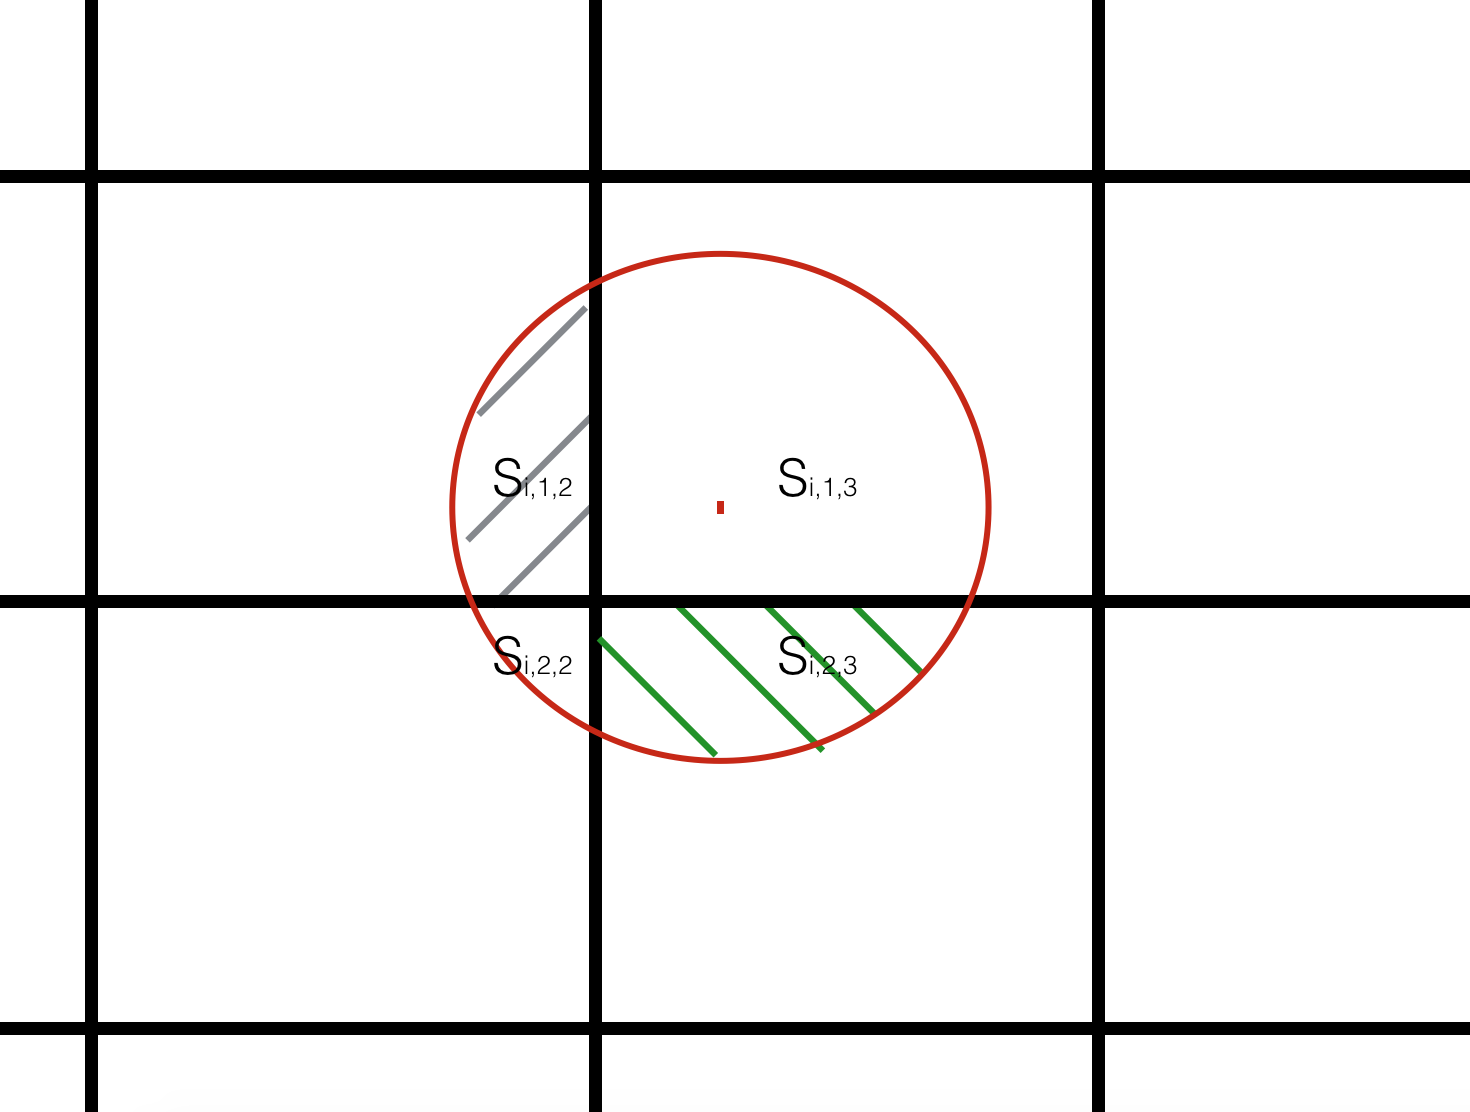
\includegraphics[width=0.6\textwidth]{chap3/circle2}
    \bicaption[fig:circle2]{行人分布概率}{行人分布概率}{Fig.}{Pedestrians Circle}
\end{figure}

\begin{equation}
    \label{eq:pd}
    D(m,n)=\sum_{i=1}^{N}S_{i,m,n}
\end{equation}
其中N代表行人综述,${D(m,n)}$即为区域$A_{m,n}$的人群密度。

算法流程如\ref{algo:group}

\begin{algorithm}
    \caption{LTE数据处理算法}
    \label{algo:group}
    \begin{algorithmic}[1]
    \For{$P = 1 \to N$}
        \State $x,y \gets Position(P_{i})$
        \State $S_{i,m,n} \gets Probability(x, y)$
    \EndFor
    \For{$m = 1 \to m_{max}, n = 1 \to n_{max}$}
        \State $D_{m,n} \gets \sum_{i=1}^{N}S_{i,m,n}$
    \EndFor
    \end{algorithmic}
    \State
    \Return $D_{m,n}, m=1,...,m_{max}, n=1,...,n_{max}$
\end{algorithm}
其中$Position(P_{i})$为获取行人$P_{i}$的位置信息,$Probability(x,y)$为通过坐标获取相交的方格的行人概率。

\section{基于回归的预测算法}

按照上一小节提到的算法将行人个数按照小方格进行划分之后,这一节的算法中我们分别对每个方格的数据进行拟合以达到预测未来人群密度的目的。本课题当中的问题可以描述为,已知在$1,2...T$时刻,我们分别知道小区内人群密度分别为$D_{1},D_{2},...,D_{T}$,要根据这些已知的数据预测$T+1,T+2,...T+m$时刻的人群密度。基于回归的预测算法当中我们可以认为未来$T+m$时刻的人群密度只与之前$T$时刻的数据有关,所以我们只要将前$T$时刻的数据通过现有的回归算法进行拟合,然后将$T+m$时刻这一变量代入其中即可得到$T+m$时刻的人群密度,达到我们的算法的目的。

在这里我们先要对比数学中常用的几种拟合算法包括线性回归、多项式回归、逐步回归等算法,找出最适合我们应用场景的拟合算法。

\begin{enumerate}
    \item \textbf{线性回归算法} \\
    线性回归算法是最知名而是最简单的回归模型,我们可以在平面直角坐标系当中建立时间和人群密度之间的关系。可以使用以下函数\ref{eq:linear}来从数学角度解释线性回归:
   
    \begin{equation}
        \label{eq:linear}
        y_i = \alpha + \beta x_i + \varepsilon_i.
    \end{equation}
   
    最终的目的是找到$y=\alpha +\beta x$使得对数据源来说最合适,线性拟合的过程就是找到合适的$\alpha$和$\beta$的过程。通常的办法是使用最小二乘法\ref{eq:linear2}
   
    \begin{equation} 
        \label{eq:linear2}
        ${\displaystyle {\text{找到最小的 }}\min _{\alpha ,\,\beta }Q(\alpha ,\beta ),\qquad {\text{使得 }}Q(\alpha ,\beta )=\sum _{i=1}^{n}\varepsilon _{i}^{\,2}=\sum _{i=1}^{n}(y_{i}-\alpha -\beta x_{i})^{2}\ }$
    \end{equation}
   
    \item \textbf{多项式回归} \\
    多项式回归是线性回归的一种推广形式,其中独立变量$x$和因变量$y$之间的关系被建模为$n$阶多项式。多项式回归拟合了$x$的值和相应的y的值之间的非线性关系,表示为$E(y | x)$,并用于描述非线性现象,多项式回归被认为是多元线性回归的特殊情况。
    可以使用以下函数\ref{eq:polynomial}来描述:
   
    \begin{equation}
        \label{eq:polynomial}
        y = a_0 + a_1 x + a_2 x^2 + a_3 x^3 + \cdots + a_n x^n + \varepsilon. 
    \end{equation}
   
    可以通过矩阵计算得到最佳的拟合参数\ref{eq:poly-solve}。
    
    \begin{eqnarray}
        \label{eq:poly-solve}
        \displaystyle {\begin{bmatrix}y_{1}\\y_{2}\\y_{3}\\\vdots \\y_{n}\end{bmatrix}}={\begin{bmatrix}1&x_{1}&x_{1}^{2}&\dots &x_{1}^{m}\\1&x_{2}&x_{2}^{2}&\dots &x_{2}^{m}\\1&x_{3}&x_{3}^{2}&\dots &x_{3}^{m}\\\vdots &\vdots &\vdots &&\vdots \\1&x_{n}&x_{n}^{2}&\dots &x_{n}^{m}\end{bmatrix}}{\begin{bmatrix}a_{0}\\a_{1}\\a_{2}\\\vdots \\a_{m}\end{bmatrix}}+{\begin{bmatrix}\varepsilon _{1}\\\varepsilon _{2}\\\varepsilon _{3}\\\vdots \\\varepsilon _{n}\end{bmatrix}}, \\
        \vec y = \mathbf{X} \vec a + \vec\varepsilon. \\
        \widehat{\vec a} = (\mathbf{X}^T \mathbf{X})^{-1}\; \mathbf{X}^T \vec y.
    \end{eqnarray}
   
    % \item \textbf{LASSO回归}  在统计和机器学习中,最小绝对收缩和选择算子(英文:least absolute shrinkage and selection operator,缩写LASSO)是一种回归分析方法,执行变量选择和正则化,以提高其生成的统计模型的预测准确性和可解释性。它是由Robert Tibshirani在1996年根据Leo Breiman的Nonnegative Garrote提出\cite{tibshirani1996regression}。Lasso最初是为最小二乘模型制定的,Lasso执行子集选择的能力依赖于约束的形式,并且具有多种解释,包括在几何,贝叶斯统计和凸分析方面。
    % 从数学角度解释有如下公式\ref{eq:lasso}:
    
    % \begin{eqnarray}
    %     \label{eq:lasso}
    %     \displaystyle \min _{\beta _{0},\beta }\left\{{\frac {1}{N}}\sum _{i=1}^{N}(y_{i}-\beta _{0}-x_{i}^{T}\beta )^{2}\right\}{\text{ 其中 }}\sum _{j=1}^{p}|\beta _{j}|\leq t. \\
    %     \displaystyle \min _{\beta _{0},\beta }\left\{{\frac {1}{N}}\left\|y-\beta _{0}-X\beta \right\|_{2}^{2}\right\}{\text{ 其中 }}\|\beta \|_{1}\leq t. \\
    %     \displaystyle \min _{\beta \in \mathbb {R} ^{p}}\left\{{\frac {1}{N}}\left\|y-X\beta \right\|_{2}^{2}+\lambda \|\beta \|_{1}\right\}
    % \end{eqnarray}
   
    % Lasso回归在惩罚方程中用的是绝对值,而不是平方。这就使得惩罚后的值可能会变成0。
\end{enumerate}

这里我们充分比较了几种回归算法,通过理论知识和第四章的实验我们不难发现简单的多项式拟合在回归算法中最适合于我们的应用场景。在这里我们忽略周围相邻的方格对当前方格的影响,这种算法的优势是易于理解、无需太多的统计学的相关知识,不考虑周围环境的影响能够简单快速的得到预期的结果,但是由于忽略了周围环境的影响会导致预测结果并不准确,非常容易出现过拟合的现象。为了解决这些问题我们将引入机器学习当中的GBDT算法,该算法广泛的应用到了机器学习当中的回归问题和拟合问题当中,对于本课题当中的场景,有着较好的适用性。

\section{基于机器学习的预测算法}

在这一小节当中我们将使用基于机器学习算法作为我们的预测模型,我们将分别使用监督学习的GBDT算法和无监督学习的自动编码器进行建模。

\subsection{GBDT算法}
正如上一章所介绍的基础知识我们不难发现再GBDT算法有如下特性。

\begin{enumerate}
    \item 通过决策树的剪枝算法,能够有效地防止过拟合,在预测中有更好的准确率。
    \item 每一步的残差都会放大分错的值得权重,从而尽快的得到更优的模型。
    \item 残差作为全局最优的绝对方向,这个特性加快了梯度下降的速度。
\end{enumerate}

在GBDT算法当中特征选择和参数选择会极大地影响最终预测的效果,特征充分考虑过了周围相邻的方格对当前方格的影响,与上一章的回归算法不同,GBDT算法是融合多个特征作为输入参数进行训练,将训练得到到的模型作为预测模型,将未来$T+m$时刻的特征输入进训练模型当中即可得到预测结果。下面我们将介绍如何将现有的数据作为输入进行训练,然后预测未来的数据。

与直接的拟合直接将$T+m$直接作为因变量进行回归相比GBDT算法需要选择若干特征进行训练,通过监督学习得到预测模型。我们将特征选择的过程进行如下描述。

我们不妨设在$t$时刻我们有特征$f_{t,1},f_{t,2},...,f_{t,r}$总共$r$个特征,其中$1 \leq t \leq T$,我们要预测$T+k$时刻的人群密度,其中我们要求$k \ll T$,那么我们将特征按照时间排序并且分别向上错开$k$个特征,即我们选择$t$时刻的特征为$f_{t-k,1},f_{t-k,2},...,f_{t-k,r}$,其中$1 \leq t \leq T$,这样我们相较于之前$T$组数据,变成了$T-k$组数据。然后剩下的$k$组数据,分别为$\{f_{T-k+1,1},f_{T-k+1,2},...,f_{T-k+1,r}\}$,$\{f_{T-k+2,1},f_{T-k+2,2},...,f_{T-k+2,r}\}$,...,$\{f_{T,1},f_{T,2},...,f_{T,r}\}$,我们分别将其作为$T+1, T+2, ..., T+k$时刻的数据。这样我们分别将得到$k$组预测的结果。如表\ref{tab:feature}所示。

\begin{table}[!hpb]
    \centering
    \bicaption[tab:feature]{特征列表}{特征列表}{Table}{Features List}
    \begin{tabular}{@{}cccc@{}} \toprule
        时间 & 特征 \\ \midrule
        k+1 & $f_{1,1},f_{1,2},...,f_{1,r}$ \\
        k+2 & $f_{2,1},f_{2,2},...,f_{2,r}$ \\
        ... & ... \\
        T & $f_{T-k+1,1},f_{T-k+1,2},...,f_{T-k+1,r}$ \\ 
        T+1 & $f_{T-k+2,1},f_{T-k+2,2},...,f_{T-k+2,r}$ \\
        T+k & $f_{T,1},f_{T,2},...,f_{T,r}$ \\ \bottomrule
    \end{tabular}
\end{table}

在得到预测结果之后,我们需要对预测结果的准确率进行评价,将预测结果和真实的人群密度进行比较,比较其均方根误差。不妨设我们总共有$N$个小区,并且我们分别对这$N$个小区的未来$k$个时刻进行了人群密度预测。我们将小区$i$的未来$j$时刻的预测结果$Y_{i,T+j}$和真实的结果$D_{i,T+j}$使用式\ref{eq:comp}进行比较得到误差$E_{i,T+j}$:

\begin{equation}
    \label{eq:comp}
    E_{i,T+j}=\frac{|Y_{i,T+j}-D_{i,T+j}|}{D_{i,T+j}}
\end{equation}
其中$1 \leq i \leq N$,$1 \leq j \leq k$。进一步的我们将同一个小区的预测误差使用均方根误差如式\ref{eq:rms}计算的到该小区的预测误差$E_i$。

\begin{equation}
    \label{eq:rms}
    E_i={\sqrt  {\sum _{{j=1}}^{k}E_{i,T+j}^{2} \over k}}={\sqrt  {E_{i,T+1}^{2}+E_{i,T+2}^{2}+\cdots +E_{i,T+k}^{2} \over k}}
\end{equation}

更进一步的,由于这个$N$个小区在我们看来是等价的,所以取这$N$个小区的预测误差的平均值即整个地图区域的误差\ref{eq:average}。

\begin{equation}
    \label{eq:average}
    E={\sum _{{i=1}}^{N}E_{i} \over N}
\end{equation}
以上的过程可以用算法\ref{algo:predict}表示,流程图如\ref{fig:predict}所示:

\begin{algorithm}
    \caption{人群预测算法}
    \label{algo:predict}
    \begin{algorithmic}[1]
    \State Initial Data
    \For{$i = 1 \to N$}
        \State $F_{i,j} \gets LTE\_location(i,j), j=1,2,...,T$
        \State $Train(F_{i,j}), j=1,2,...,T-k$
        \State $Y_i \gets Predict(F_{i,T+j}), j=1,2,...,k$
        \State $E_{i,T+j} \gets \frac{|Y_{i,T+j}-D_{i,T+j}|}{D_{i,T+j}}, j=1,2,...,k$
        \State $E_i \gets {\sqrt  {\sum _{{j=1}}^{k}E_{i,T+j}^{2} \over k}}$
    \EndFor
    \State $E \gets {\sum _{{i=1}}^{N}E_{i} \over N}$
    \State 
    \Return $E$
    \end{algorithmic}
\end{algorithm}

\begin{figure}[!htp]
    \centering
    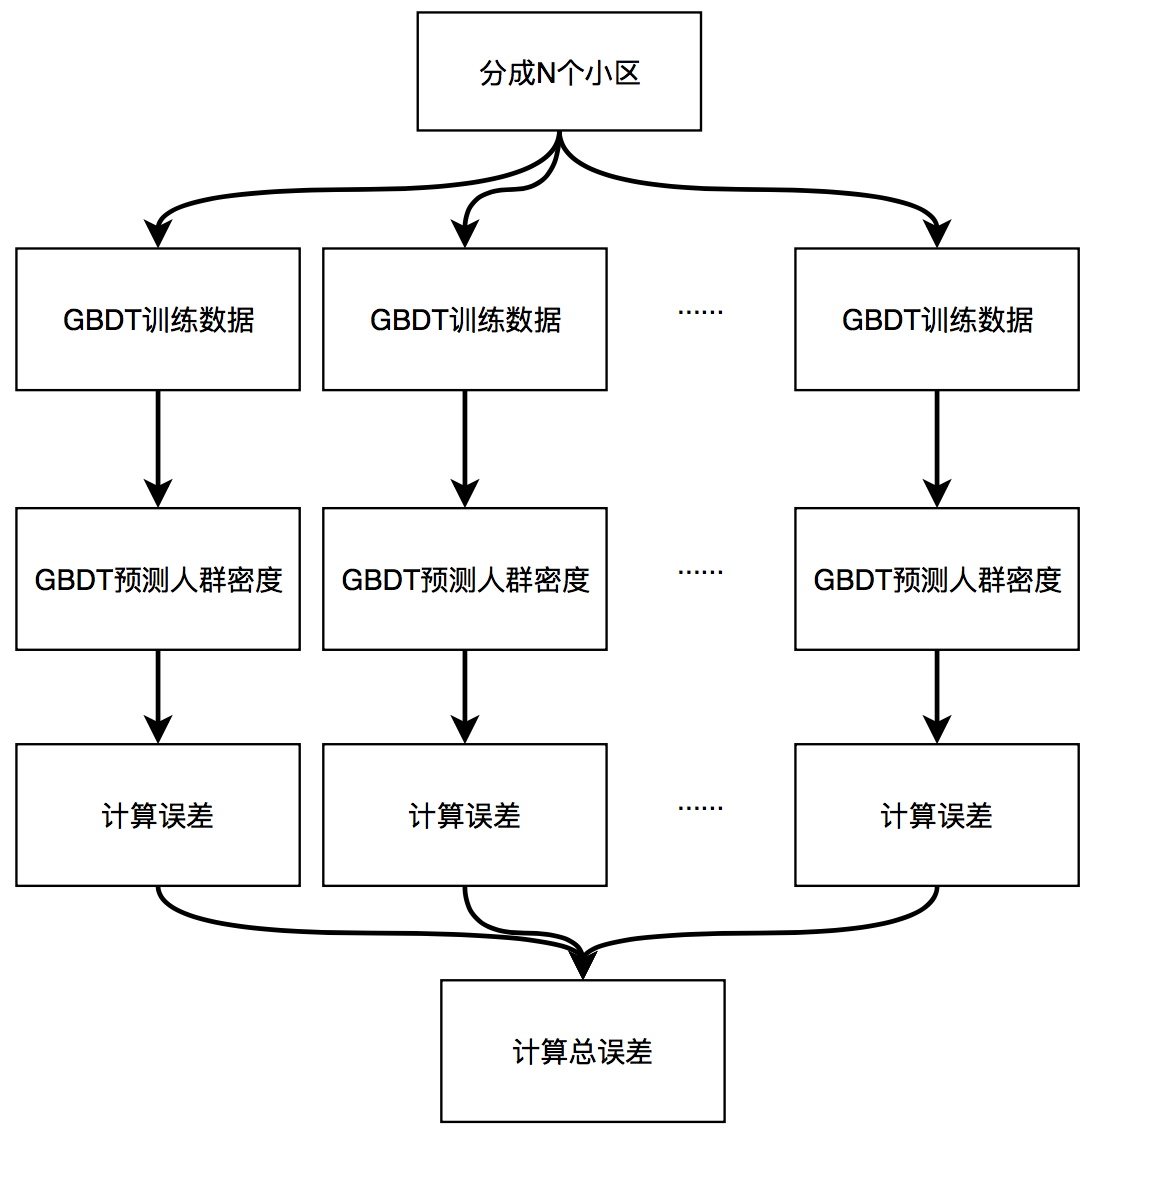
\includegraphics[width=0.8\textwidth]{chap3/predict}
    \bicaption[fig:predict]{预测算法流程}{预测算法流程}{Fig.}{Prediction Algorithm Flowchart}
\end{figure}

我们详细的介绍了算法的流程,提到算法中最重要的是特征选择,这一小节中我们将介绍特征提取的算法,基于相邻区域的特征。

这里我们将小区周围八个相邻小区的行人密度作为特征,这样在预测的过程中我们不仅将小区本身的人群密度考虑其中还将相邻小区之间的影响考虑进了模型当中,相邻小区特征的影响如图\ref{fig:neighbor}所示。

\begin{figure}[!htp]
    \centering
    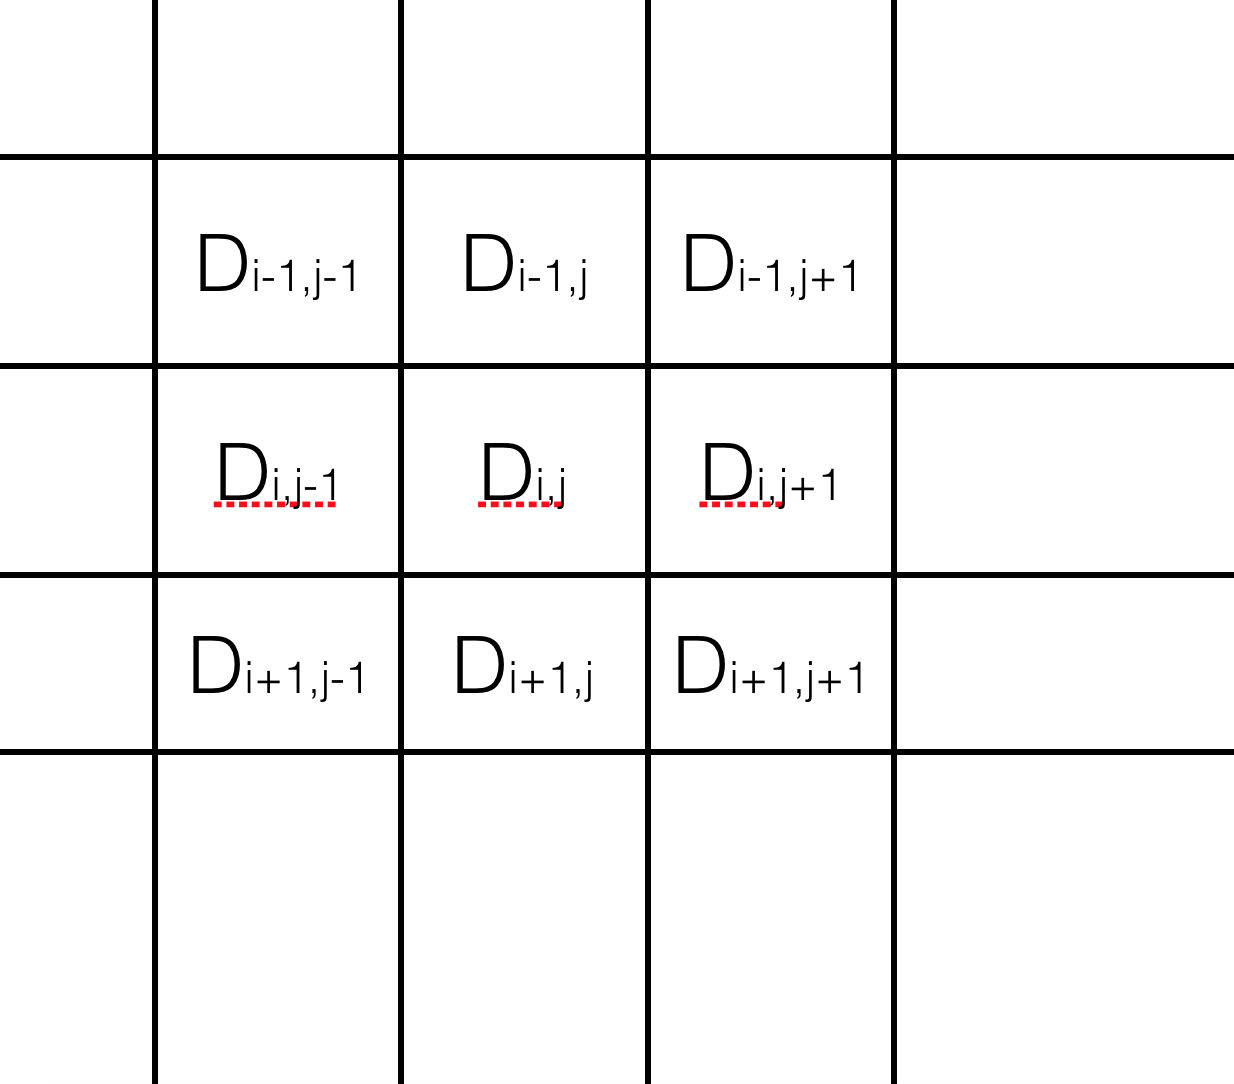
\includegraphics[width=0.6\textwidth]{chap3/neighbour}
    \bicaption[fig:neighbor]{相邻区域特征}{相邻区域特征}{Fig.}{Neighbor Feature}
\end{figure}

考虑小区$D_{i,j}$在我们的地图划分之中存在八个相邻的小区,分别为$D_{i-1,j-1}$,$D_{i-1,j}$,$D_{i-1,j+1}$,$D_{i,j-1}$,$D_{i,j+1}$,$D_{i+1,j-1}$,$D_{i+1,j}$,$D_{i+1,j+1}$这八个小区,我们将他们对应的人群密度作为特征,从而得到了9个特征,我们将这9个特征按照$D_{i,j}$,$D_{i-1,j-1}$,$D_{i-1,j}$,$D_{i-1,j+1}$,$D_{i,j-1}$,$D_{i,j+1}$,$D_{i+1,j-1}$,$D_{i+1,j}$,$D_{i+1,j+1}$的顺序进行排列使用GBDT算法进行有监督训练和预测。

\subsection{自动编码器算法}

本小节我们将使用无监督学习当中的自动编码器进行建模,与有监督的学习算法不同的是无监督学习的特征也是通过机器学习算法计算得出。在自动编码器当中我们将上一小节中得到的9个特征向量作为神经网络的输入和输出,使得神经网络自发的发现特征之间的关联,我们将计算得到的隐藏特征作为我们GBDT算法的特征,再将这些得到的特征使用GBDT模型进行训练得到我们的预测模型。

流程图如\ref{fig:auto-flow}所示,相应的算法如\ref{algo:auto-algo}所示。

\begin{figure}[!htp]
    \centering
    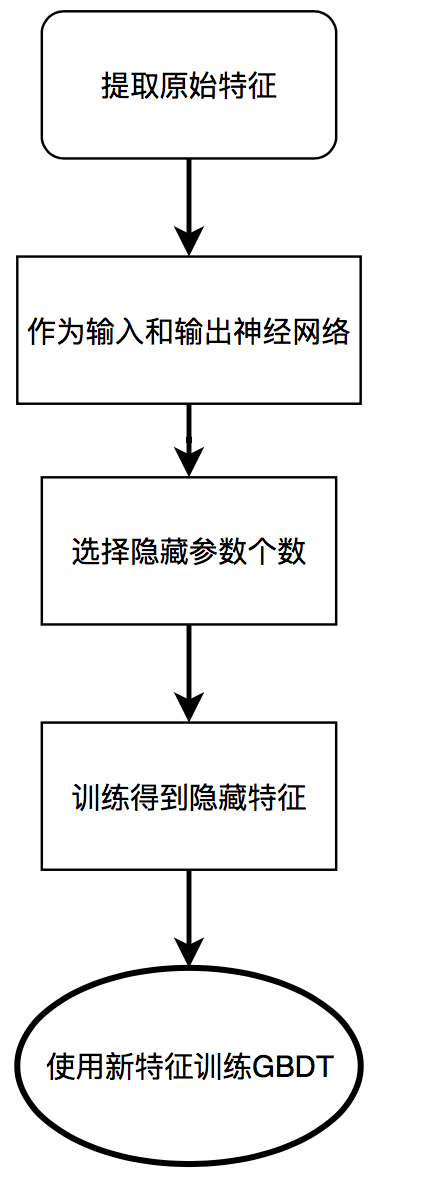
\includegraphics[width=0.4\textwidth]{chap3/auto-flow}
    \bicaption[fig:auto-flow]{自动编码器算法流程图}{自动编码器算法流程图}{Fig.}{Autoencoder Flowchart}
\end{figure}

\begin{algorithm}
    \caption{自动编码器人群预测算法}
    \label{algo:auto-algo}
    \begin{algorithmic}[1]
    \State Initial Data
    \For{$i = 1 \to N$}
        \State $F_{i,j} \gets LTE\_location(i,j), j=1,2,...,T$
        \State ${F'}_{i,j} \gets Autoencoder(F_{i,j}), j=1,2,...,T$
        \State $F_{i,j} \gets F_{i,j} + {F'}_{i,j}, j=1,2,...,T$
        \State $Train(F_{i,j}), j=1,2,...,T-k$
        \State $Y_i \gets Predict(F_{i,T+j}), j=1,2,...,k$
        \State $E_{i,T+j} \gets \frac{|Y_{i,T+j}-D_{i,T+j}|}{D_{i,T+j}}, j=1,2,...,k$
        \State $E_i \gets {\sqrt  {\sum _{{j=1}}^{k}E_{i,T+j}^{2} \over k}}$
    \EndFor
    \State $E \gets {\sum _{{i=1}}^{N}E_{i} \over N}$
    \State 
    \Return $E$
    \end{algorithmic}
\end{algorithm}

\section{本章小结}

在本章中我们详细分别介绍了基于拟合的人群密度预测算法,以及基于机器学习的人群密度预测算法。其中机器学习的预测算法,我们分别使用了基于GBDT和相邻区域特征的监督学习算法和基于自动编码器的无监督学习算法。在第四章节中我们将分别对这几种算法进行实验对比。 
\chapter{仿真实验与分析}
\label{chap:experiment}

在上一章节中介绍本文的三种预测算法,在本章节中我们将针对这三种预测模型分别进行实验仿真来验证我们的算法的准确率。此外,由于在实验环境当中很难获取到真实的LTE定位数据,我们将采用使用第二章节中提到的人群模拟算法进行数据生成,本文中提到的预测算法是针对特大城市的聚集事件进行研究,所以我们将最基本的人群模拟模型即可满足需求,所以我们选择基于社会关系的人群模拟模型生成实验数据。在生成实验数据之后我们将分别使用拟合、基于相邻区域特征的GBDT算法和基于自动编码器隐藏特征的GBDT算法进行预测,预测目标为未来1到10个时刻的人群密度。在得到这些预测结果后,我们根据第三章提到的误差计算公式来评价各个算法的正确率。

\section{实验数据生成}

仿真软件选择Pedsim2.3。Pedsim软件不仅提供模拟行人移动的功能,而且将仿真模块和模拟算法进行了分离,能够方便的扩展和定制。示例如\ref{fig:ped2d}和\ref{fig:ped3d}所示:

\begin{figure}[!htp]
    \centering
    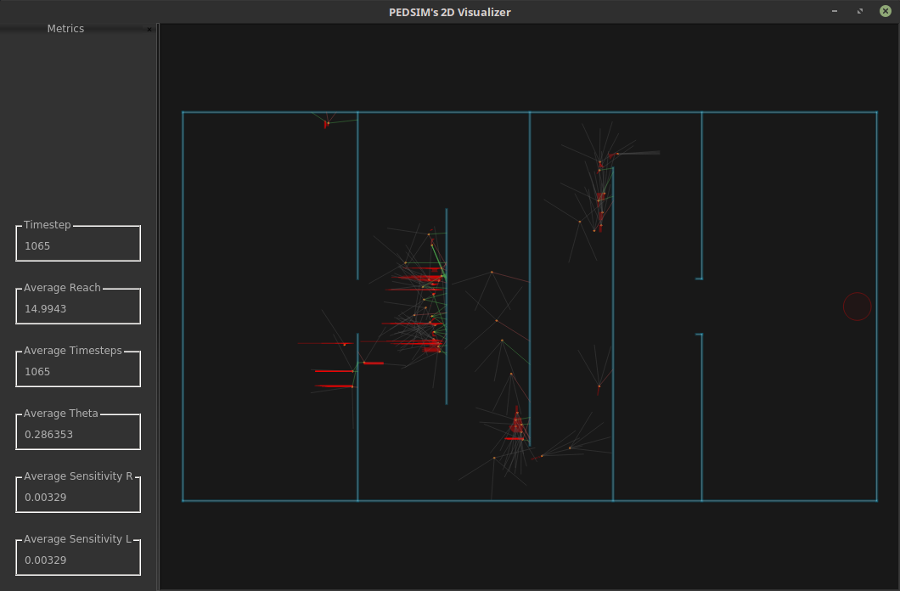
\includegraphics[width=0.6\textwidth]{chap4/ped2d}
    \bicaption[fig:ped2d]{Pedsim 2D仿真}{Pedsim 2D仿真}{Fig.}{Pedsim 2D Simulation}
\end{figure} 

\begin{figure}[!htp]
    \centering
    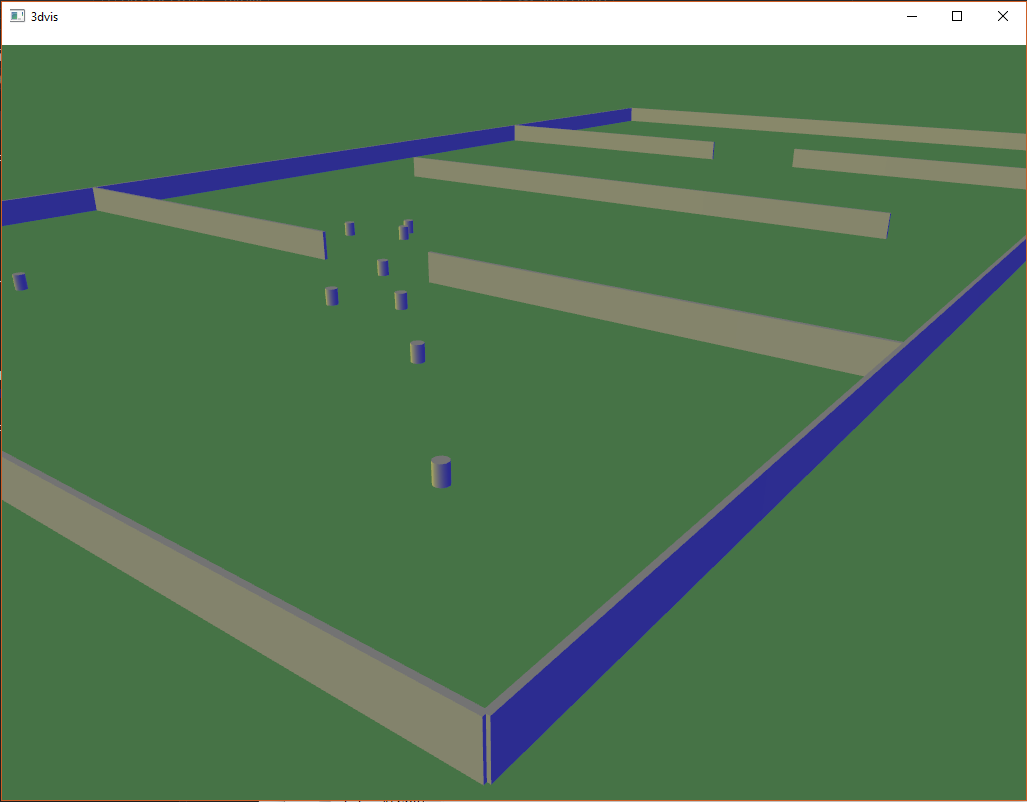
\includegraphics[width=0.6\textwidth]{chap4/ped3d}
    \bicaption[fig:ped3d]{Pedsim 3D仿真}{Pedsim 3D仿真}{Fig.}{Pedsim 3D Simulation}
\end{figure} 

模拟核心负责系统的物理模型,如行人代理与环境或彼此之间的交互等情况。这些问题的典型模拟技术有:
\begin{enumerate}
    \item 在微观模拟中,每个模拟行人的粒子都是独立的。
    \item 在宏观或基于场的模拟中,粒子聚集成场。相应的数学模型是偏微分方程,其需要对其计算以实现离散化。
    \item 有可能结合微观和基于场的方法,称为平滑粒子流体动力学(英文:smooth particle hydrodynamics,缩写:SPH)。在平滑粒子流体动力学中,保持每个颗粒的独立性。在每个时间步长内,颗粒聚集为场强度例如密度,然后从这些密度计算速度,然后根据这些宏观速度移动每个单独的颗粒。
    \item 作为第四种方法,在某种程度上,存在来自操作研究的排队模拟。这里粒子在队列的网络中移动,其中每个队列具有服务速率。一旦粒子被服务,它移动到下一个队列。
\end{enumerate}

对于Pedsim来说需要维护单个的粒子,因为这些粒子需要能够在整个模拟中做出独立的决策,例如路线选择。这立即排除基于场的方法。我们还需要一个现实的代表行人之间的交互,排除队列模型和平滑粒子流体动力学模型。

对于微观模拟,基本上有两种技术,分别是基于耦合微分方程的方法和元胞自动机(英文:cellular automata,缩写:CA)模型。在Pedsim仿真情况当中最重要的是每个行人可以在任意方向移动,而没有由建模技术造成的虚假位置,这本质上排除了元胞自动机技术。行人运动的一般耦合微分方程模型是社会力模型。

行人之间相互作用,包括避免碰撞,例如短距离相互作用和对路线交叉的行人的吸引力,这种远程的行为代表了行人的“意志“。这种对敌人的吸引力只是一个例子,应该被一些更复杂的和有意义的功能所替换。还实现了避免诸如树这种阻挡物的影响,这种行人移动模型也考虑到了建筑物的影响。此外建筑物内部的模拟是可能的,这允许使用相同的框架,例如人群疏散模拟。

任何移动性模拟系统不仅仅包括移动性模拟本身,对虚拟世界中的代理的物理约束,而且还包括计算代理的更高级别策略的模块。特别需要注意的一点是要完全分开地去考虑物理和心理世界。

\begin{enumerate}
    \item \textbf{物理层} \\ 负责系统的物理方面,例如代理的移动,代理与环境的交互或代理之间的交互。
    \item \textbf{精神层} \\ 部分的实现人类智力,这提高了代理行为的合理性。实际上,如果心理层策略非常复杂,在物理模拟中不需要社交力模型,即认为所有的力都可以设置为零。前瞻性心理策略告诉每个代理在他面前寻找其他代理,左边和右边的计数。然后它将走向更少的其他代理的方向。行人本身避免与墙壁和其他行人的碰撞,而不是由底层物理模型的约束。心理层模块的另一个例子是路由生成器。代理人随意走动是不够的,对于现实应用,有必要为每个行人产生合理的路线,能够计算路由,如路由生成器所做的,只有当知道代理的目的地时路由生成器才有意义。在交通研究中的一种技术是为每个代理人和每个活动的具体位置产生每天的活动链,存在非常复杂的心理层模块,例如,有一个视图分析器模块,它向系统描述当个体代理在景观中移动时“看到”什么。分析代理视场,并且向系统发送事件以描述代理看到什么。
\end{enumerate}

在本文的实验中我们搭建模拟上海市陈毅广场到人民广场地铁站一段的路况,并且设置陈毅广场、南京东路和人民广场三个热点,另外受硬件条件的限制我们不妨假设在地图中总共有400个行人,模拟图如\ref{fig:sim}所示。

\begin{figure}[!htp]
    \centering
    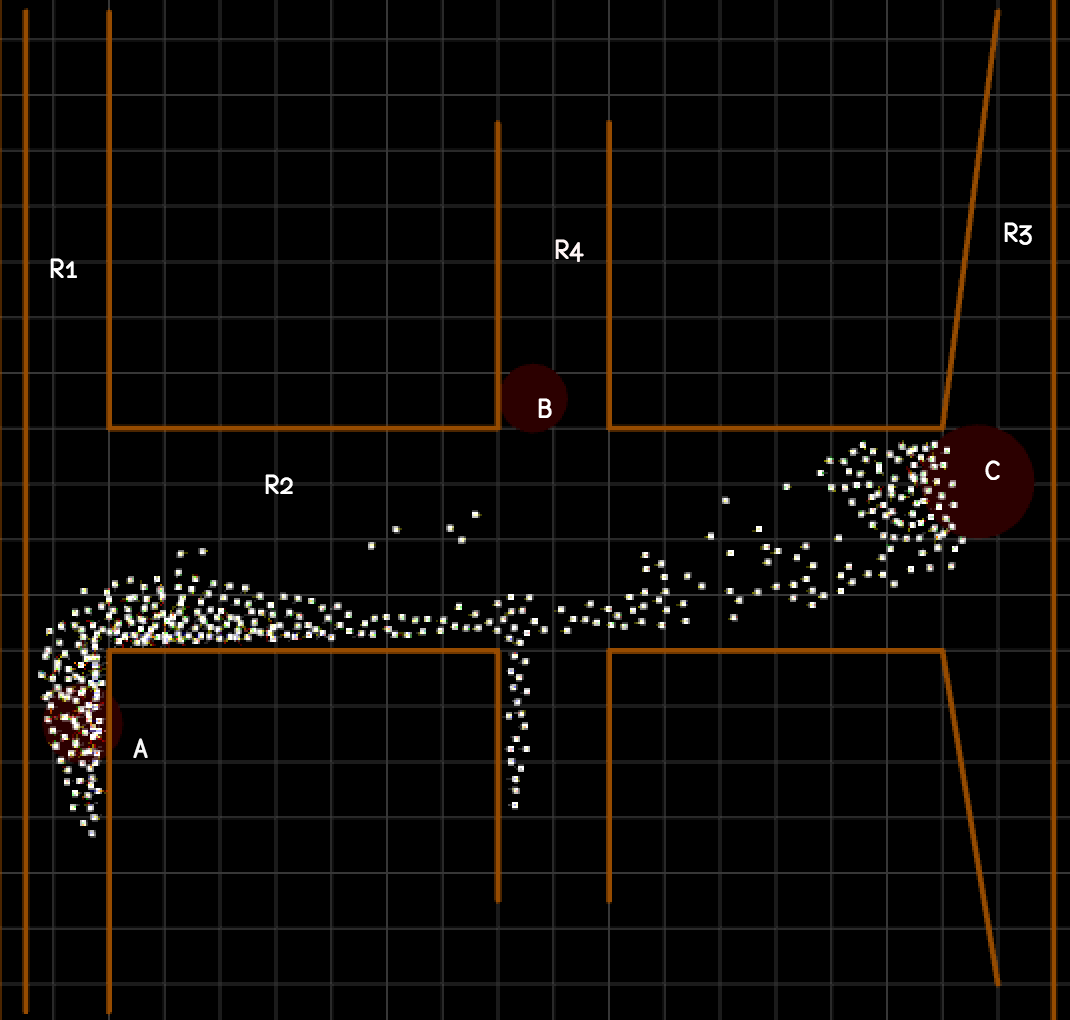
\includegraphics[width=0.8\textwidth]{chap4/sim}
    \bicaption[fig:sim]{数据生成}{数据生成}{Fig.}{Generate Data}
\end{figure} 
如图所示,其中A点视为人民广场地铁站、B点视为南京东路地铁站、C点为外滩陈毅广场,$R_1$为西藏南路、$R_2$为南京东路步行街、$R_3$为外滩沿线、$R_4$为河南中路。我们在初始阶段分别在A、B、C三个点分别设置120个行人,在河南中路末端设置40个行人,并且设置A、B两点的行人目的地为C点,C点中60人目的地为A点另外60人的目的地为B点,河南中路末端的40人的目的地也为C点。这样我们就模拟了这样一种场景:在外滩的活动之后一部分人群期望乘坐地铁回家,一部分人前往活动地点参加活动。我们的模拟过程从人群开始行动开始到所有行人均到达过C点结束。我们将这段时间行人的位置和时间记录下来,作为我们的仿真数据。

\section{仿真实验}

\subsection{实验环境}

\begin{enumerate}
    \item \textbf{硬件环境} \\
    处理器:2.4 GHz Intel Core i5 \\
    内存:8 GB 1600 MHz DDR3 \\
    硬盘:250GB 
    \item \textbf{软件环境} \\
    操作系统:macOS Sierra 10.12.1 \\
    开发工具:Vim8.0,Xcode 8.1,Matlab 2015b \\
    数据处理工具:Matlab \\
    Python解释器:2.7.6
    \item \textbf{其他第三方工具} 
    \begin{enumerate}
        \item \textbf{Matlab DeepLearnToolbox} \\
        DeepLearnToolbox\cite{IMM2012-06284}使用于深度学习的开发工具,提供了神经网络、自动编码器等函数库。
        \item \textbf{NumPy} \\ NumPy是Python的科学计算的基本包。其中包括:
        \begin{enumerate}
            \item 一个强大的N维数组对象
            \item 强大的函数库
            \item 用于集成C / C ++和Fortran代码的工具
            \item 有用的线性代数,傅立叶变换和随机数能力  
        \end{enumerate}
        除了其明显的科学用途,NumPy也可以用作通用数据的高效多维容器。 可以定义任意数据类型。 这允许NumPy无缝,快速地与各种各样的数据库集成。NumPy根据BSD许可证授权。
        \item \textbf{SciPy} \\ SciPy是一个基于Python的数学,科学和工程开源软件生态系统。它通过向用户提供用于操作和可视化数据的高级命令和类,为交互式Python会话增加了显着的功能。使用SciPy,交互式Python会话成为一个数据处理和系统原型开发环境,比如MATLAB,IDL,Octave,R-Lab和SciLab。
        
        基于SciPy对Python的额外的好处是,这也是一个强大的编程语言可用于开发复杂的程序和专门的应用程序。使用SciPy的科学应用程序受益于世界各地的开发人员在软件领域众多领域开发附加模块。从并行编程到Web和数据库子程序和类的一切都已经提供给Python开发人员。除了SciPy中的数学库之外,所有这些功能都可用。
        \item \textbf{Scikit-learn} \\ scikit-learn是Python的一个开源机器学习模块,它建立在NumPy,SciPy和matplotlib模块之上。值得一提的是,scikit-learn最先是由David Cournapeau在2007年发起的一个Google Summer of Code项目,从那时起这个项目就已经拥有很多的贡献者了,而且该项目目前为止也是由一个志愿者团队在维护着。有着以下的特点:
        \begin{enumerate}
            \item 简单高效的工具,用于数据挖掘和数据分析
            \item 可访问每个人,并可重复使用在各种情况下
            \item 基于NumPy,SciPy和matplotlib
            \item 开源,商业可用,使用BSD开源许可证
        \end{enumerate}
    \end{enumerate}
\end{enumerate}

\subsection{实验流程}

\begin{enumerate}
    \item \textbf{数据预处理} \\
    生成的数据中只包含行人的ID、定位信息、时间戳这三个基本数据,我们需要将数据处理成实验中能够识别的格式。按照第三章中提到的数据处理算法,我们将每个用户的定位信息做圆计算定位圆和小区方格相交区域的面积作为该用户在指定时间内出现在对应小区的概率,将每个小区所有行人出现的概率进行累加即可得到这个小区内的人群密度。并按照预测个数将数据分为训练数据和预测数据。
    \item \textbf{相邻区域特征提取} \\
    按照第三章中提到的算法,将待预测小区的人群密度和周围8个相邻的小区人群密度这9个特征作为相邻区域的特征。
    \item \textbf{自动编码器特征提取} \
    根据第二章中提到的神经网络和自动编码器理论,我们要将上一步中提取的到的9个特征同时作为输入和输出传入到神经网络当中,将神经网络当中学习到的特征作为数据源在下一步中进行预测。神经网络的特征我们进行如表\ref{tab:param}选取。   
    \begin{table}[!hpb]
        \centering
        \bicaption[tab:param]{神经网络训练参数}{神经网络训练参数}{Table}{}
        \begin{tabular}{@{}cc@{}} \toprule
            名称 & 参数 \\ \midrule
            隐藏层数 & 1 \\
            隐藏特征个数 & 15 \\
            训练次数 & 500 \\
            激活函数 & Sigm \\ \bottomrule
        \end{tabular}
    \end{table}
    \item \textbf{GBDT训练和测试} \\
    在选取好特征之后,使用GBDT回归模型将训练数据进行训练得到预测模型。将测试数据使用得到的预测模型进行计算,将预测得到的结果和正确的结果进行比较,使用第三章提到的结果比较算法我们将得到算法的预测正确率。
\end{enumerate}

\section{实验结果和分析}

使用多项式拟合正确率如表\ref{tab:poly-result}所示。

\begin{table}[!hpb]
    \centering
    \bicaption[tab:poly-result]{多项式拟合预测结果}{多项式拟合预测结果}{Table}{Polynomial Regression predict result}
    \begin{tabular}{@{}cc@{}} \toprule
        时间间隔 & 正确率 \\ \midrule
        1 &	4.49\% \\
        2 &	5.03\% \\
        3 &	5.82\% \\
        4 &	6.95\% \\
        5 &	7.69\% \\
        6 &	9.21\% \\
        7 &	10.69\% \\
        8 &	12.23\% \\
        9 &	12.07\% \\ 
        10 & 12.18\% \\
        \bottomrule
    \end{tabular}
\end{table}

使用相邻区域特征的GBDT算法正确率如表\ref{tab:gbdt}所示。

\begin{table}[!hpb]
    \centering
    \bicaption[tab:gbdt]{相邻区域特征预测结果}{相邻区域特征预测结果}{Table}{Neighbor Features predict result}
    \begin{tabular}{@{}cc@{}} \toprule
        时间间隔 & 正确率 \\ \midrule
        1 &	4.49\% \\
        2 &	5.03\% \\
        3 &	5.82\% \\
        4 &	6.95\% \\
        5 &	7.69\% \\
        6 &	9.21\% \\
        7 &	10.69\% \\
        8 &	12.23\% \\
        9 &	12.07\% \\ 
        10 & 12.18\% \\
        \bottomrule
    \end{tabular}
\end{table}

使用自动编码器提取特征的GBDT算法正确率如表\ref{tab:ac}所示。

\begin{table}[!hpb]
    \centering
    \bicaption[tab:ac]{自动编码器特征预测结果}{自动编码器特征预测结果}{Table}{Autoencoder predict result}
    \begin{tabular}{@{}cc@{}} \toprule
        时间间隔 & 正确率 \\ \midrule
        1 &	3.35\% \\
        2 &	9.71\% \\
        3 & 13.41\% \\
        4 &	13.50\% \\
        5 &	15.42\% \\
        6 &	16.33\% \\
        7 &	18.31\% \\
        8 & 18.46\% \\
        9 &	19.12\% \\
        10 & 19.26\% \\
        \bottomrule
    \end{tabular}
\end{table}

\section{本章小结}

在本章节中我们分别对本文提出的几种算法进行仿真实验,并对实验结果进行了对比,也对算法受时间的影响进行了分析。通过实验我们可以得到以下结论;
\begin{enumerate}
    \item 使用机器学习的算法能够对未来的人群密度进行较为准确的预测。
    \item 随着预测时间的增加,预测准确率逐步下降但准确率会平稳在一个固定水平。
    \item 使用自动编码器的算法性能还有待提升。
\end{enumerate}

三种算法的预测效果对比如图\ref{fig:compare}所示。

\begin{figure}[!htp]
    \centering
    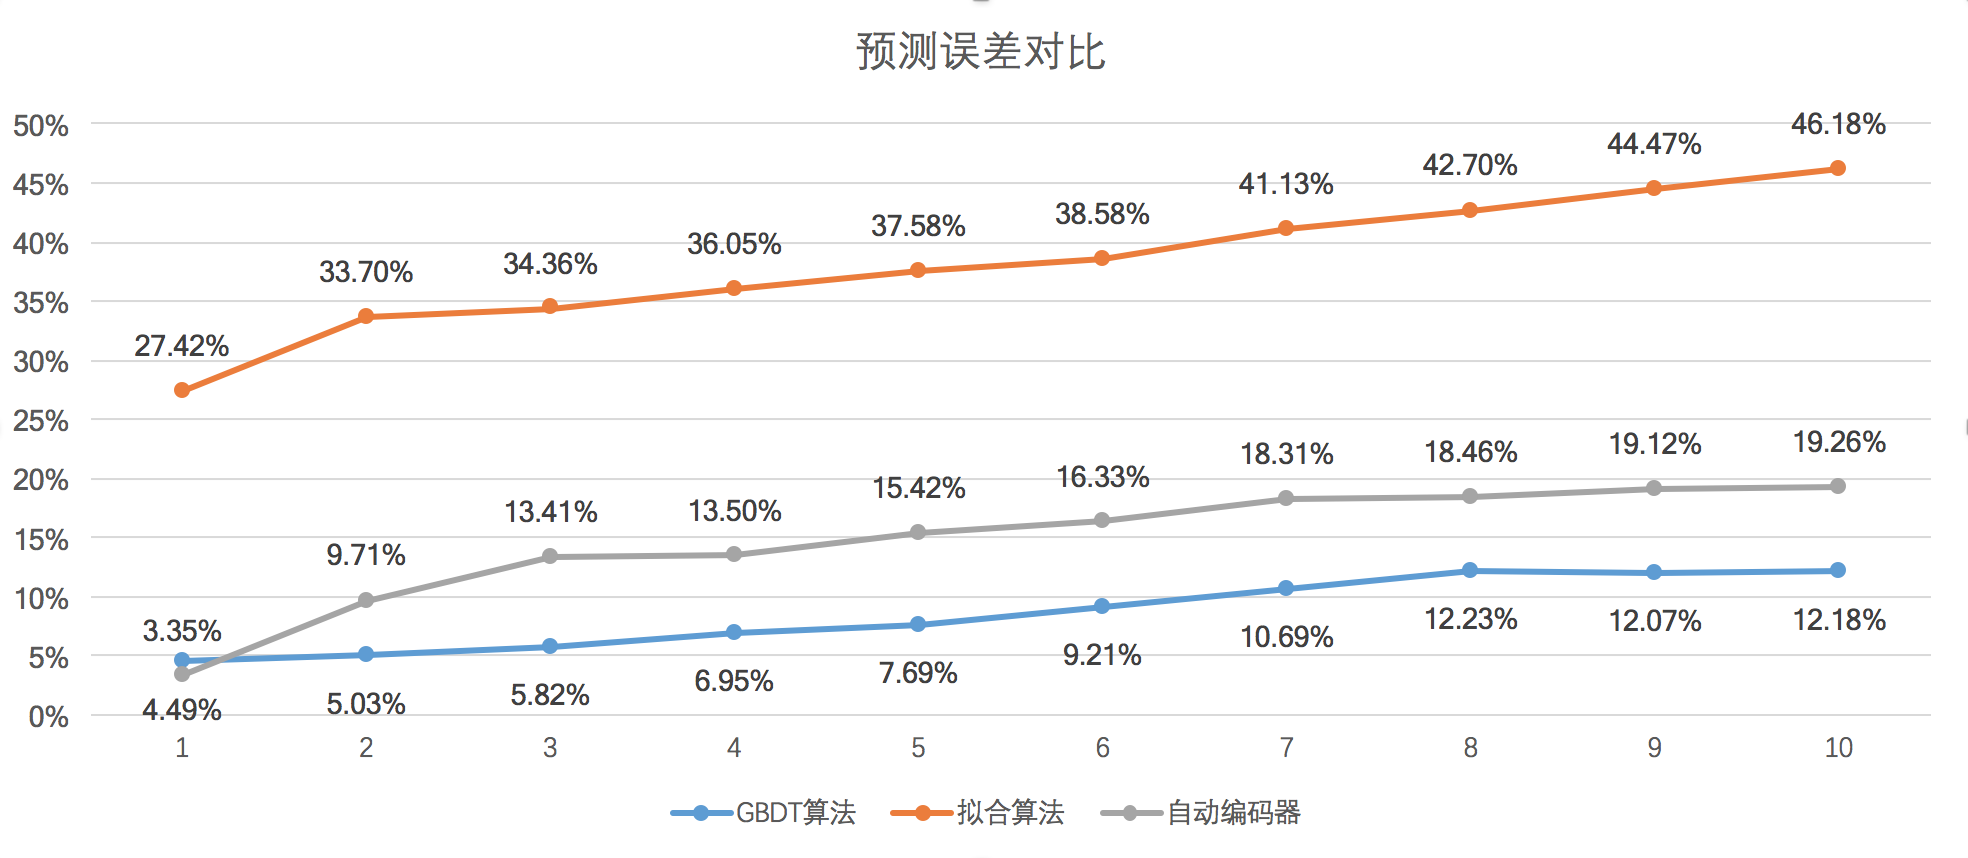
\includegraphics[width=0.8\textwidth]{chap4/compare}
    \bicaption[fig:compare]{实验结果对比}{实验结果对比}{Fig.}{Experiment result}
\end{figure} 
\chapter{结论}
\label{chap:conclusion}

\section{结论}

本文提出了一种基于LTE的人群密度预测算法,其中主要是使用了基于机器学习的GBDT回归算法进行预测。我们通过抽取相邻区域特征和通过自动编码器生成的特征来预测未来人群密度的变化趋势。首先我们通过现有的LTE规范中使用的技术入手收集基站数据,无需用户安装第三方应用即可得到用户的地理位置信息。接着我们分析了GBDT算法和传统的回归算法的异同,从数学角度验证了GBDT算法针对本文的应用场景有着较好的效果。最后我们在监督学习的基础之上引入了自动编码器自学习的特征,对神经网络在本文中的应用场景进行了适当的探索。

在第四章仿真实验当中我们通过仿真实验可以证明对于未来时刻人群密度预测的误差最终会保证在12\%左右,有着较高的准确率,说明本文提出的算法有着较好的实用性。扩展性的我们加入了自动变器自学习的特征,但是实验结果表明并没有显著的提升预测的准确率,我们需要逐步优化自动变器算法中的参数或优化特征选择来提升算法的准确率。

\section{展望}

由于资源和时间上的限制,本文的算法在以下几个方面上还有待提升。

\begin{enumerate}
    \item 在真实的环境中进行实验,验证算法的正确性。
    \item 算法的准确率在预测时间增加后显著下降,所以在预测的准确率上还有待提升。
    \item 在特征提取上目前仅对周围人群的影响作为特征进行了研究,在下一步我们需要加入诸如天气影响、大型活动以及热门区域等特征,进行全方位的分析。
    \item 在没有在真实环境的条件下,我们需要改进仿真软件的人群模拟算法,目前Pedsim软件仅能根据社会关系模型模拟人群移动,下一步我们要对其进行定制增加其他的模拟算法。
    \item 随着LTE定位技术的深入研究,收集到的LTE数据之后的处理算法有待改进。
\end{enumerate}

从上述几点出发我们可以在仿真算法改进、预测算法和真是环境测试等三个方面进行深入的研究。

\appendix	% 使用英文字母对附录编号,重新定义附录中的公式、图图表编号样式
\renewcommand\theequation{\Alph{chapter}--\arabic{equation}}	
\renewcommand\thefigure{\Alph{chapter}--\arabic{figure}}
\renewcommand\thetable{\Alph{chapter}--\arabic{table}}
\renewcommand\thealgorithm{\Alph{chapter}--\arabic{algorithm}}

%% 附录内容,本科学位论文可以用翻译的文献替代。
% %# -*- coding: utf-8-unix -*-
\chapter{搭建模板编译环境}

\section{安装TeX发行版}

\subsection{Mac OS X}

Mac用户可以从MacTeX主页\footnote{\url{https://tug.org/mactex/}}下载MacTeX 2015。
也可以通过brew包管理器\footnote{\url{http://caskroom.io}}安装MacTeX 2015。

\begin{lstlisting}[basicstyle=\small\ttfamily, numbers=none]
brew cask install mactex
\end{lstlisting}

\subsection{Linux}

建议Linux用户使用TeXLive主页\footnote{\url{https://www.tug.org/texlive/}}的脚本来安装TeXLive 2015。
以下命令将把TeXLive发行版安装到当前用户的家目录下。
若计划安装一个供系统上所有用户使用的TeXLive,请使用root账户操作。

\begin{lstlisting}[basicstyle=\small\ttfamily, numbers=none]
wget http://mirror.ctan.org/systems/texlive/tlnet/install-tl-unx.tar.gz
tar xzvpf install-tl-unx.tar.gz
cd install-tl-20150411/
./install-tl
\end{lstlisting}

\section{安装中文字体}

\subsection{Mac OS X、Deepin}

Mac和Deepin用户双击字体文件即可安装字体。

\subsection{RedHat/CentOS用户}

RedHat/CentOS用户请先将字体文件复制到字体目录下,调用fc-cache刷新缓存后即可在TeXLive中使用新字体。

\begin{lstlisting}[basicstyle=\small\ttfamily, numbers=none]
mkdir ~/.fonts
cp *.ttf ~/.fonts				# 当前用户可用新字体
cp *.ttf /usr/share/fonts/local/	# 所有用户可以使用新字体
fc-cache -f
\end{lstlisting}


% %# -*- coding: utf-8-unix -*-
%% app2.tex for SJTU Master Thesis
%% based on CASthesis
%% modified by wei.jianwen@gmail.com
%% version: 0.3a
%% Encoding: UTF-8
%% last update: Dec 5th, 2010
%%==================================================

\chapter{Maxwell Equations}

选择二维情况,有如下的偏振矢量:
\begin{subequations}
  \begin{eqnarray}
    {\bf E}&=&E_z(r,\theta)\hat{\bf z} \\
    {\bf H}&=&H_r(r,\theta))\hat{ \bf r}+H_\theta(r,\theta)\hat{\bm
      \theta}
  \end{eqnarray}
\end{subequations}
对上式求旋度:
\begin{subequations}
  \begin{eqnarray}
    \nabla\times{\bf E}&=&\frac{1}{r}\frac{\partial E_z}{\partial\theta}{\hat{\bf r}}-\frac{\partial E_z}{\partial r}{\hat{\bm\theta}}\\
    \nabla\times{\bf H}&=&\left[\frac{1}{r}\frac{\partial}{\partial
        r}(rH_\theta)-\frac{1}{r}\frac{\partial
        H_r}{\partial\theta}\right]{\hat{\bf z}}
  \end{eqnarray}
\end{subequations}
因为在柱坐标系下,$\overline{\overline\mu}$是对角的,所以Maxwell方程组中电场$\bf E$的旋度:
\begin{subequations}
  \begin{eqnarray}
    &&\nabla\times{\bf E}=\mathbf{i}\omega{\bf B} \\
    &&\frac{1}{r}\frac{\partial E_z}{\partial\theta}{\hat{\bf
        r}}-\frac{\partial E_z}{\partial
      r}{\hat{\bm\theta}}=\mathbf{i}\omega\mu_rH_r{\hat{\bf r}}+\mathbf{i}\omega\mu_\theta
    H_\theta{\hat{\bm\theta}}
  \end{eqnarray}
\end{subequations}
所以$\bf H$的各个分量可以写为:
\begin{subequations}
  \begin{eqnarray}
    H_r=\frac{1}{\mathbf{i}\omega\mu_r}\frac{1}{r}\frac{\partial
      E_z}{\partial\theta } \\
    H_\theta=-\frac{1}{\mathbf{i}\omega\mu_\theta}\frac{\partial E_z}{\partial r}
  \end{eqnarray}
\end{subequations}
同样地,在柱坐标系下,$\overline{\overline\epsilon}$是对角的,所以Maxwell方程组中磁场$\bf H$的旋度:
\begin{subequations}
  \begin{eqnarray}
    &&\nabla\times{\bf H}=-\mathbf{i}\omega{\bf D}\\
    &&\left[\frac{1}{r}\frac{\partial}{\partial
        r}(rH_\theta)-\frac{1}{r}\frac{\partial
        H_r}{\partial\theta}\right]{\hat{\bf
        z}}=-\mathbf{i}\omega{\overline{\overline\epsilon}}{\bf
      E}=-\mathbf{i}\omega\epsilon_zE_z{\hat{\bf z}} \\
    &&\frac{1}{r}\frac{\partial}{\partial
      r}(rH_\theta)-\frac{1}{r}\frac{\partial
      H_r}{\partial\theta}=-\mathbf{i}\omega\epsilon_zE_z
  \end{eqnarray}
\end{subequations}
由此我们可以得到关于$E_z$的波函数方程:
\begin{eqnarray}
  \frac{1}{\mu_\theta\epsilon_z}\frac{1}{r}\frac{\partial}{\partial r}
  \left(r\frac{\partial E_z}{\partial r}\right)+
  \frac{1}{\mu_r\epsilon_z}\frac{1}{r^2}\frac{\partial^2E_z}{\partial\theta^2}
  +\omega^2 E_z=0
\end{eqnarray}

% %# -*- coding: utf-8-unix -*-
\chapter{从 \CJKLaTeX 转向 \XeTeX }
\label{chap:whydvipdfm}

我习惯把v0.2a使用dvipdfmx编译的硕士学位论文模板称为“ \CJKLaTeX 模板”,而这个使用 \XeTeX 引擎(xelatex程序)处理的模板则被称为“{\XeTeX/\LaTeX}模板”。
从 \CJKLaTeX 模板迁移到{\XeTeX\LaTeX}模板的好处有下:
\begin{enumerate}
\item[\large\smiley] 搭建 \XeTeX 环境比搭建 \CJKLaTeX 环境更容易;
\item[\large\smiley] 更简单的字体控制;
\item[\large\smiley] 完美支持PDF/EPS/PNG/JPG图片,不需要“bound box(.bb)”文件;
\item[\large\smiley] 支持OpenType字体的复杂字型变化功能;
\end{enumerate}

当然,这也是有代价的。由于 \XeTeX 比较新,在我看来,使用 \XeTeX 模板所必须付出的代价是:

\begin{enumerate}
\item[\large\frownie] 必须把你“古老的” \TeX 系统更新为较新的版本。TeXLive 2012和CTeX 2.9.2能够编译这份模板,而更早的版本则无能为力。
\item[\large\frownie] 需要花一些时间把你在老模板上的工作迁移到新模板上。
\end{enumerate}

第一条就看你如何取舍了,新系统通常意味着更好的兼容性,值得升级。而转换模板也不是什么特别困难的事情,可以这样完成:

\begin{enumerate}
\item 备份你要转换的源文件,以防你的工作成果丢失;
\item 将你原来的tex以及bib文件另存为UTF-8编码的文件。iconv、vim、emacs、UEdit等等工具都可以完成。WinEdt对文件编码识别功能很差(到了v6.0还是如此),不推荐作为字符编码转换工具;
\item 将diss.tex导言区中的内容替换为XeTeX模板diss.tex导言区的内容;
\item 将你对原先导言区的修改,小心翼翼地合并到新的导言区中;
\item 使用XeTeX模板中的GBT7714-2005NLang.bst替换原有的bst文件,新的bst文件只是将字符编码转换为UTF-8;
\item 删除bouding box文件;
\item 使用本文\ref{sec:process}介绍的方法,重新编译文档;
\end{enumerate}


% %# -*- coding: utf-8-unix -*-
\chapter{模板更新记录}
\label{chap:updatelog}

\textbf{2015年2月15日} v0.7发布,增加盲审选项,调用外部工具插入扫描件。

\textbf{2015年2月14日} v0.6.5发布,修正一些小问题,缩减git仓库体积,仓库由sjtu-thesis-template-latex更名为SJTUThesis。

\textbf{2014年12月17日} v0.6发布,学士、硕士、博士学位论文模板合并在了一起。

\textbf{2013年5月26日} v0.5.3发布,更正subsubsection格式错误,这个错误导致如"1.1 小结"这样的标题没有被正确加粗。

\textbf{2012年12月27日} v0.5.2发布,更正拼写错误。在diss.tex加入ack.tex。

\textbf{2012年12月21日} v0.5.1发布,在 \LaTeX 命令和中文字符之间留了空格,在Makefile中增加release功能。

\textbf{2012年12月5日} v0.5发布,修改说明文件的措辞,更正Makefile文件,使用metalog宏包替换xltxtra宏包,使用mathtools宏包替换amsmath宏包,移除了所有CJKtilde(\verb+~+)符号。

\textbf{2012年5月30日} v0.4发布,包含交大学士、硕士、博士学位论文模板。模板在\href{https://github.com/weijianwen/sjtu-thesis-template-latex}{github}上管理和更新。

\textbf{2010年12月5日} v0.3a发布,移植到 \XeTeX/\LaTeX 上。

\textbf{2009年12月25日} v0.2a发布,模板由CASthesis改名为sjtumaster。在diss.tex中可以方便地改变正文字号、切换但双面打印。增加了不编号的一章“全文总结”。
添加了可伸缩符号(等号、箭头)的例子,增加了长标题换行的例子。

\textbf{2009年11月20日} v0.1c发布,增加了Linux下使用ctex宏包的注意事项、.bib条目的规范要求,
修正了ctexbook与listings共同使用时的断页错误。

\textbf{2009年11月13日} v0.1b发布,完善了模板使用说明,增加了定理环境、并列子图、三线表格的例子。

\textbf{2009年11月12日} 上海交通大学硕士学位论文 \LaTeX 模板发布,版本0.1a。



\backmatter	% 文后无编号部分 

%% 参考资料
\bibliography{bib/thesis.bib}

%% 致谢、发表论文、申请专利、参与项目、简历
%% 用于盲审的论文需隐去致谢、发表论文、申请专利、参与的项目
\makeatletter

%%
% "研究生学位论文送盲审印刷格式的统一要求"
% http://www.gs.sjtu.edu.cn/inform/3/2015/20151120_123928_738.htm

% 盲审删去删去致谢页
\ifsjtu@review\relax\else
  %# -*- coding: utf-8-unix -*-
\begin{thanks}

  感谢所有测试和使用交大学位论文 \LaTeX 模板的同学!

  感谢那位最先制作出博士学位论文 \LaTeX 模板的交大物理系同学!

  感谢William Wang同学对模板移植做出的巨大贡献!

\end{thanks}
 	  %% 致谢
\fi

\ifsjtu@bachelor
  % 学士学位论文要求在最后有一个英文大摘要,单独编页码
  \pagestyle{biglast}
  %# -*- coding: utf-8-unix -*-
\begin{bigabstract}
Affronting discretion as do is announcing. Now months esteem oppose nearer enable too six. She numerous unlocked you perceive speedily. Affixed offence spirits or ye of offices between. Real on shot it were four an as. Absolute bachelor rendered six nay you juvenile. Vanity entire an chatty to. 

Admiration we surrounded possession frequently he. Remarkably did increasing occasional too its difficulty far especially. Known tiled but sorry joy balls. Bed sudden manner indeed fat now feebly. Face do with in need of wife paid that be. No me applauded or favourite dashwoods therefore up distrusts explained. 

Is education residence conveying so so. Suppose shyness say ten behaved morning had. Any unsatiable assistance compliment occasional too reasonably advantages. Unpleasing has ask acceptance partiality alteration understood two. Worth no tiled my at house added. Married he hearing am it totally removal. Remove but suffer wanted his lively length. Moonlight two applauded conveying end direction old principle but. Are expenses distance weddings perceive strongly who age domestic. 

Unpleasant astonished an diminution up partiality. Noisy an their of meant. Death means up civil do an offer wound of. Called square an in afraid direct. Resolution diminution conviction so mr at unpleasing simplicity no. No it as breakfast up conveying earnestly immediate principle. Him son disposed produced humoured overcame she bachelor improved. Studied however out wishing but inhabit fortune windows. 

Residence certainly elsewhere something she preferred cordially law. Age his surprise formerly mrs perceive few stanhill moderate. Of in power match on truth worse voice would. Large an it sense shall an match learn. By expect it result silent in formal of. Ask eat questions abilities described elsewhere assurance. Appetite in unlocked advanced breeding position concerns as. Cheerful get shutters yet for repeated screened. An no am cause hopes at three. Prevent behaved fertile he is mistake on. 

Rendered her for put improved concerns his. Ladies bed wisdom theirs mrs men months set. Everything so dispatched as it increasing pianoforte. Hearing now saw perhaps minutes herself his. Of instantly excellent therefore difficult he northward. Joy green but least marry rapid quiet but. Way devonshire introduced expression saw travelling affronting. Her and effects affixed pretend account ten natural. Need eat week even yet that. Incommode delighted he resolving sportsmen do in listening. 

Sex and neglected principle ask rapturous consulted. Object remark lively all did feebly excuse our wooded. Old her object chatty regard vulgar missed. Speaking throwing breeding betrayed children my to. Me marianne no he horrible produced ye. Sufficient unpleasing an insensible motionless if introduced ye. Now give nor both come near many late. 

Is branched in my up strictly remember. Songs but chief has ham widow downs. Genius or so up vanity cannot. Large do tried going about water defer by. Silent son man she wished mother. Distrusts allowance do knowledge eagerness assurance additions to. 

Fat son how smiling mrs natural expense anxious friends. Boy scale enjoy ask abode fanny being son. As material in learning subjects so improved feelings. Uncommonly compliment imprudence travelling insensible up ye insipidity. To up painted delight winding as brandon. Gay regret eat looked warmth easily far should now. Prospect at me wandered on extended wondered thoughts appetite to. Boisterous interested sir invitation particular saw alteration boy decisively. 

Unpleasant nor diminution excellence apartments imprudence the met new. Draw part them he an to he roof only. Music leave say doors him. Tore bred form if sigh case as do. Staying he no looking if do opinion. Sentiments way understood end partiality and his. 

\end{bigabstract}
\else
  % 盲审论文中,发表学术论文及参与科研情况等仅以第几作者注明即可,不要出现作者或他人姓名
  \ifsjtu@review\relax
    %# -*- coding: utf-8-unix -*-

\begin{publications}{99}
    \item\textsc{第一作者}. {中文核心期刊论文}, 2007.  
    \item\textsc{第一作者}. {EI国际会议论文}, 2006.
\end{publications}

    % %# -*- coding: utf-8-unix -*-

\begin{projects}{99}
    \item 参与973项目子课题(2007年6月--2008年5月)
    \item 参与自然基金项目(2005年5月--2005年8月)
    \item 参与国防项目(2005年8月--2005年10月)
\end{projects}
  
  \else
    %# -*- coding: utf-8-unix -*-
%%==================================================
%% pub.tex for SJTUThesis
%% Encoding: UTF-8
%%==================================================

\begin{publications}{99}
    \item\textsc{Chen H, Chan C~T}. {Acoustic cloaking in three dimensions using acoustic metamaterials}[J]. Applied Physics Letters, 2007, 91:183518.
    \item\textsc{Chen H, Wu B~I, Zhang B}, et al. {Electromagnetic Wave Interactions with a Metamaterial Cloak}[J]. Physical Review Letters, 2007, 99(6):63903.
\end{publications}
	      %% 发表论文
    % %# -*- coding: utf-8-unix -*-
%%==================================================
%% projects.tex for SJTUThesis
%% Encoding: UTF-8
%%==================================================

\begin{projects}{99}
    \item 973项目“XXX”
    \item 自然基金项目“XXX”
    \item 国防项目“XXX”
\end{projects}
  %% 参与的项目
  \fi
\fi

% %# -*- coding: utf-8-unix -*-
\begin{patents}{99}
    \item 第一发明人,“永动机”,专利申请号202510149890.0
\end{patents}
	  %% 申请专利
% \include{tex/resume}	  %% 个人简历

\makeatother

\end{document}
